\documentclass{beamer}
\usepackage{colortbl}
\usepackage{etex}
\input{/home/mnattaf/Documents/input_latex/usepackage.tex}
\usepackage[T1]{fontenc}
\usepackage[utf8]{inputenc}
\usepackage[english]{babel}
\usepackage{pgfpages}
\usepackage{blindtext}
\usepackage[lang=en]{templateLAAS}

% \addtobeamertemplate{footline}{\insertframenumber/\inserttotalframenumber}

\setbeamersize{text margin left=25pt}
\setbeamersize{text margin right=25pt}
\input{/home/mnattaf/Documents/input_latex/newcommand.tex}


\title{Scheduling Under Energy Constraints}
\author{Margaux NATTAF}
\institute{LAAS-CNRS Toulouse

  Université Paul Sabatier Toulouse}


\setbeamertemplate{itemize item}[ball]
\setbeamertemplate{itemize subitem}[triangle]
\setbeamertemplate{itemize subsubitem}[circle]

\newcolumntype{M}[1]{>{\centering\arraybackslash}m{#1}}

\begin{document}

{\canvasspecial
  \begin{frame}
    \vspace{1.5cm}
    \begin{flushleft}
      {\Large \bf \color{bleuLAAS}SCHEDULING UNDER ENERGY CONSTRAINTS}
      
      \vspace{0.3cm}
      \small \color{bleuLAAS!90} defended by Margaux NATTAF

      October 18, 2016
    \end{flushleft}
    \vspace{0.5cm}

    {\footnotesize  \color{bleuLAAS!80}
      Supervised by Christian ARTIGUES \& Pierre LOPEZ}

    \vspace{1.5cm}
    \begin{flushright} \color{bleuLAAS!70}
      \scriptsize LAAS-CNRS, Toulouse

      Université Paul Sabatier, Toulouse
    \end{flushright}
  \end{frame}}

\setcounter{framenumber}{0}

\section{Introduction}

\begin{frame}{What is {\it Scheduling}?}
  \vfill
  \begin{block}{Larousse}
    {\bf \color{bleuLAAS} Scheduling: }organization, methodical arrangement of the different
    element of a set, of the  different phases of a fabrication.
  \end{block}
  \vfill
\pause
  \begin{block}{Cambridge}
    {\bf  \color{bleuLAAS}  Scheduling: }the job or activity of planning the times at which particular tasks will be done or events will happen.
  \end{block}
  \vfill  
\pause
  \begin{block}{Wikipedia}
    A {\bf  \color{bleuLAAS}  scheduling} problem consists in organizing the realization of
    tasks through time, given time constraints (setup time, precedence)
    and constraints on the availability of required resources.
  \end{block}
  \vfill
\end{frame}

\begin{frame}{What is {\it Scheduling}?}
\vspace{0.3cm}
  \begin{block}{My thesis}
    The {\bf  \color{bleuLAAS} scheduling} theory aims at computing {\bf activities execution
      start/end times} subject to a certain number of {\bf
      constraints} in order to optimize an {\bf objective}.    
  \end{block}
  \vspace{0.6cm}
  \begin{description}
\pause
  \item[activities :]  courses, landing/taking off, step in a
    construction project... 
    \vspace{0.2cm}
\pause
  \item[constraints :]
    \begin{itemize}
    \item temporal $\rightarrow$ deadline, precedence, setup...
    \item resource $\rightarrow$ availability, nature... 
    \end{itemize}
\pause
    \vspace{0.2cm}
  \item[objective :] resource consumption, total cost, makespan,
    tardiness... 
    \vspace{0.2cm}
  \end{description}
\end{frame}

% \begin{frame}{Application example: Timetable}
  
%   {\usebeamercolor[fg]{item} activities: } set of courses\\[0.2cm]

% \onslide<2->{
%           {\usebeamercolor[fg]{item} temporal constraints: } Precedence relationship: lecture before
%             exercise, Analysis 1 before Analysis 2...\\[0.2cm]
% }

% \onslide<3->{
%          {\usebeamercolor[fg]{item} resource constraints: }rooms, teachers, additional material...\\[0.2cm]}

%          \vfill
%       \begin{center}
%       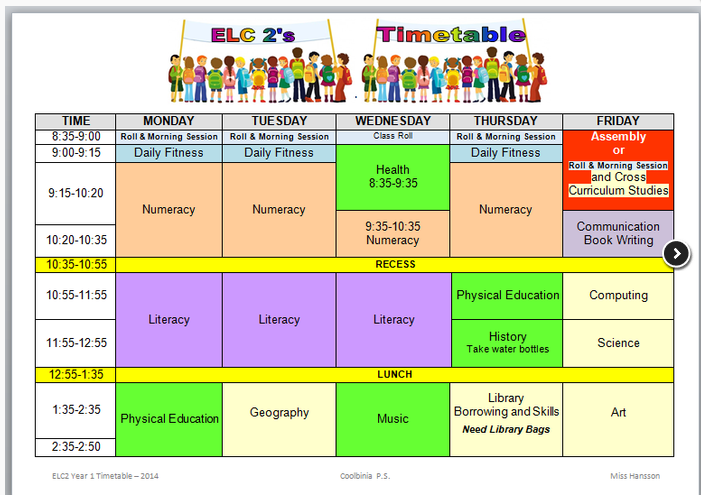
\includegraphics[scale=0.25]{figures/timetable.png}
%     \end{center}
% \vspace{-0.5cm}    
% \end{frame}


% \begin{frame}{Resource and activity characteristics}
%     \begin{tikzpicture}\tikzstyle{every node} = [align=center]
%       \node at (0,0) {\bf \phantom{ain} activity types \phantom{ons}};

%       \draw[thick,->] (2.5,0) -- (3.3,0.3);
%       \draw[thick,->] (2.5,0) -- (3.3,-0.3);

%       \node at (4.9,0.3)  {preemptive};
%       \node at (5.25,-0.3) {non-preemptive};
%     \end{tikzpicture}
% \vfill
% \pause
%   \begin{tikzpicture}\tikzstyle{every node} = [align=center]
%     \node[text width=4cm] at (0,0) { \bf resource types };

%     \draw[thick,->] (2.5,0) -- (3.3,0.5);
%     \draw[thick,->] (2.5,0) -- (3.3,-0.5);

%     \draw[white] (0,0);
%     \node at (5.7,0.5)  {disjunctive/cumulative};
%     \node at (4.9,0)  {\footnotesize rooms/workers};
%     \node at (6,-0.5) {renewable/non-renewable};
%     \node at (5,-1)  {\footnotesize machines/money};
%   \end{tikzpicture}
%   \vfill
% \pause
%   \begin{tikzpicture}\tikzstyle{every node} = [align=center]
%     \node at (0,0) {};
%     \node[text width=4cm] at (0,0) { \bf resource constraints };

%     \draw[thick,->] (2.5,0) -- (3.3,0.3);
%     \draw[thick,->] (2.5,0) -- (3.3,-0.3);

%     \node at (5.7,0.3)  {resource usage {\footnotesize (tasks)}};
%     \node at (6.3,-0.3) {resource availability {\footnotesize (resource)}};
%   \end{tikzpicture}
%   \vspace{-1cm}
% \end{frame}

\begin{frame}
  \frametitle{The Cumulative Scheduling Problem} 
\vspace{0.1cm}
 \textbf{Inputs : }
\vspace{0.15cm}
  \begin{itemize}
  \item a set ${\cal A}=\{1,\dots ,n\}$ of non-preemptive tasks
\vspace{0.15cm}
    \item a cumulative and renewable resource available in quantity $B$
\vspace{0.15cm}
    \item<2-> for each task:
      \vspace{-1cm}
      \begin{columns}
        \hfill
        \begin{column}{0.36\linewidth}
          \begin{itemize}
          \item<2-> \footnotesize  a processing time $p_i$
          \item<3-> \footnotesize a resource consumption $b_i$ 
          \item<4-> \footnotesize a release date $est_i$ and a deadline $let_i$ 
          \end{itemize}
        \end{column}
        \begin{column}{0.7\linewidth}
          \centering
          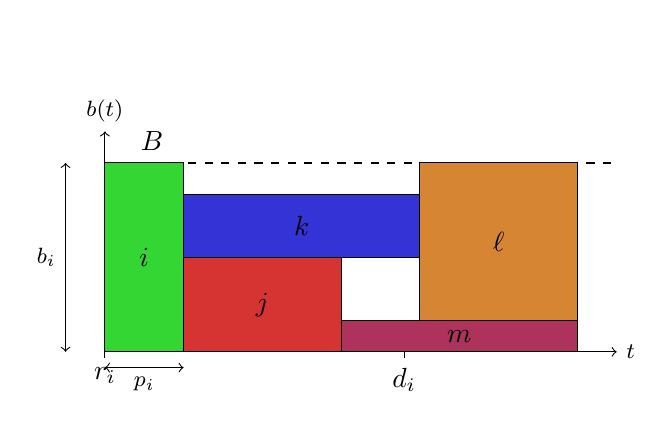
\begin{tikzpicture}
  [yscale=0.4]
  \node at (0,10) {};

  \node[label={[shift={(-0.4,-0.5)}]}] (O) at (0,0) {};
  \draw[fill=red!80!black!80] (1,0) rectangle (3,3)   node[midway] {$j$};
  \draw[dashed,thick] (0,6)   -- (6.5,6);
  \node at (0.6,6.7)  {$B$};
    \draw[<->] (0,-0.5) -- (1,-0.5) node[midway,below] {\footnotesize $p_i$};
    \draw[<->] (-0.5,0) -- (-0.5,6) node[midway,left] {\footnotesize $b_{i}$};
  
  \draw (0,0) -- (0,-0.2) node[below] {$r_i$};
  \draw (3.8,0) -- (3.8,-0.2) node[below] {$d_i$};
  
  \draw[fill=green!80!black!80] (0,0) rectangle (1,6)   node[midway] {$i$};
  \draw[fill=blue!80!black!80] (1,3) rectangle (4,5)   node[midway] {$k$};
  \draw[fill=orange!80!black!80] (4,1) rectangle (6,6)   node[midway] {$\ell$};
  \draw[fill=purple!80!black!80] (3,0) rectangle (6,1)   node[midway] {$m$};
  \draw[->] (O.center) -- (0,7) node[above] {\footnotesize $b(t)$};
  \draw[->] (O.center) -- (6.5,0) node[right] {\footnotesize $t$};


\end{tikzpicture}

      \end{column} 
    \end{columns}
  \end{itemize}
\vspace{-0.5cm}
\onslide<6->{
\textbf{Application : }
\vfill
  \begin{itemize}
  \item electricity consumption cannot exceed a certain level.
  \end{itemize}}
\end{frame}


 \begin{frame}{ CuSP preemptive}
  
\end{frame}

\begin{frame}
  \frametitle{Limitations}
 \vspace{0.5cm}
  \begin{itemize}
  \item {Limitation} : tasks have fixed duration and resource consumption
    \vfill
  \item<2-> But, in practice, it is not always the case\\
   \end{itemize}
  \vspace{1cm}
  \begin{columns}
\hfill
    \begin{column}{0.45\linewidth}
      \centering
      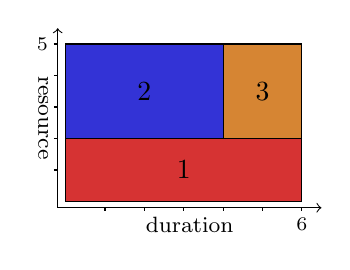
\begin{tikzpicture}
        [xscale=0.5,yscale=0.4]
        \node (O) at (0,0) {};
          \draw[fill=red!80!black!80] (0,0) rectangle (6,2) node[midway] {$1$};
          \draw[fill=blue!80!black!80] (0,2) rectangle (4,5) node[midway] {$2$};
          \draw[fill=orange!80!black!80] (4,5) rectangle (6,2) node[midway] {$3$};
          \draw[->](-0.2,-0.2) -- (-0.2,5.5) node[midway,below,rotate=-90] {\footnotesize resource};
        
        \draw[->] (-0.2,-0.2) -- (6.5,-0.2) node[midway,below]
        {\footnotesize duration};
        \foreach \i in {1,...,5}{
          \draw (-0.3,\i) -- (-0.2,\i);
          \draw (\i, -0.3) -- (\i,-0.2);
}
\onslide<3->{
          \draw (-0.3,5) -- (-0.2,5) node[left] {\scriptsize  $5$};
          \draw (6, -0.3) -- (6,-0.2) node[below] {\scriptsize  $6$};}
      \end{tikzpicture}
    \end{column}
    \hfill
    \begin{column}{0.45\linewidth}
      \centering
      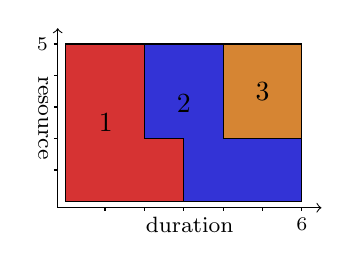
\begin{tikzpicture}
        [xscale=0.5,yscale=0.4]
        \node (O) at (0,0) {};
        \onslide<3->{
         \onslide<4->{ 
           \path[draw,fill=blue!80!black!80] (3,2) -- (2,2) -- (2,5) -- (4,5) -- (4,2) -- (6,2) --
           (6,0) --(3,0); 
           \path[draw] (0,0) -- (0,5) -- (2,5) -- (2,2) -- (3,2)
           node[above=0.2cm] {$2$} -- (3,0)-- cycle; 
            \draw[fill=orange!80!black!80] (4,2) rectangle (6,5) node[midway] {$3$};}
          \draw[->] (-0.2,-0.2) -- (6.5,-0.2) node[midway,below] {\footnotesize duration};

          \path[draw,fill=red!80!black!80] (0,0) node[above=1cm,right=0.3cm] {$1$}-- (0,5) -- (2,5) -- (2,2) -- (3,2) -- (3,0)-- cycle;
          \draw[->](-0.2,-0.2) -- (-0.2,5.5)
          node[midway,below,rotate=-90] {\footnotesize resource};
        \foreach \i in {1,...,5}{
          \draw (-0.3,\i) -- (-0.2,\i);
          \draw (\i, -0.3) -- (\i,-0.2);}

          \draw (-0.3,5) -- (-0.2,5) node[left] {\scriptsize $5$};
          \draw (6, -0.3) -- (6,-0.2) node[below] {\scriptsize  $6$};}
      \end{tikzpicture}
    \end{column}
\hfill
  \end{columns}
\end{frame}


\begin{frame}{Motivating Problem
 {\small \it \color{gray!50!black!50} [Artigues et al., 2013]}} 
  \vfill
\begin{block}{}
  \begin{center}
    {\bf \large   pipe-manufacturing plant}
    
    \vspace{0.2cm}
    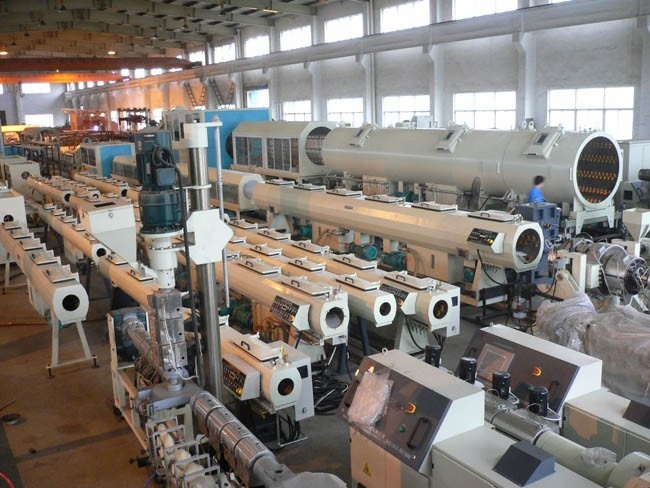
\includegraphics[scale=0.1]{pipe.jpg}

  \begin{tikzpicture}[yscale=.6]
    \node (O) at (0,0) {};
    \draw[-latex,ultra thick, bleuLAAS!100!black!50] (O.center) -- (-3,-1.5);
    \draw[-latex,ultra thick, bleuLAAS!100!black!50] (O.center) -- (0,-1.5);
    \draw[-latex,ultra thick, bleuLAAS!100!black!50] (O.center) -- (3,-1.5);

 \node[draw] at (-3.4,-2.1) {drawing mill}; 
    \node[draw] at (3.5,-2.1) {pipe-tubing};

    \node[draw] at (0,-2.1) {\textbf<4>{foundry}};
  \end{tikzpicture}
  \end{center}
\end{block}
\vfill
\pause
  \begin{itemize}
  \item melting and heating use a {\bf HUGE} quantity of energy
\vfill
\pause
  \item $\Rightarrow$ high electricity cost:
    \begin{itemize}
    \item total energy consumed
    \item penalty for power overrun
    \end{itemize}
  \end{itemize}
\end{frame}



\begin{frame}
  \frametitle{Motivating Problem 
 {\small \it \color{gray!50!black!50} [Artigues et al., 2013]}}
  \vfill
  \begin{columns}
    \begin{column}{0.5\linewidth}
      \begin{itemize}
      \item a set of melting jobs
\pause
        \vspace{0.4cm}
      \item melting operation has variable duration\\
        {\small (depending of the power given + may vary over time)}
\pause
         \vspace{0.4cm}
      \end{itemize}     
    \end{column}
    \hfill 
 \begin{column}{0.4\linewidth}
       \onslide<1->{  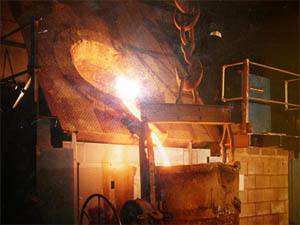
\includegraphics[width=0.8\linewidth]{figures/induction.jpg}}
    \end{column}
  \end{columns}
  \vfill
  \begin{itemize}
  \item upper and lower bound on the power given \\
    {\small(operational and physical consideration)}
    \vspace{0.4cm}
\pause
  \item electrical power limitation\\
    {\small(electrical overrun cost)}
  \end{itemize}
\end{frame}

\begin{frame}
  \frametitle{Literature review}
  \begin{itemize}
    \vfill
  \item {\bf Cumulative Scheduling Problem (CuSP)},
    {\color{gray!50!black!50} \it [Erschler \& Lopez, 1990] }, {\color{blue!80!black!80} fixed resource consumption}
    \vfill
\pause
  \item {\bf Fully elastic scheduling}, {\color{gray!50!black!50} \it [Baptiste et al., 1999]}, {\color{blue!80!black!80} no upper and lower bound on the consumption}
    \vfill
\pause
  \item {\bf Variable Intensity}, {\color{gray!50!black!50} \it [Kis, 2005]}, {\color{blue!80!black!80} no lower bound on the consumption}
    \vfill  
\pause
  \item {\bf Scheduling with continuous resource}, {\color{gray!50!black!50}\it [Blazewicz et al., 2006]}, {\color{blue!80!black!80}  no upper and lower bound}
    \vfill
\pause
  \item {\bf Multimode RCPSP}, {\color{gray!50!black!50}\it [De Reyck
      et al., 1998]},
    {\color{blue!80!black!80} tasks have rectangular shape}
  \end{itemize}
  \vfill
\end{frame}


\begin{frame}{The CECSP : definition }
   Generalization of the CuSP
   \begin{itemize}
     \vfill
\pause
   \item Duration $p_i$ $\leftrightarrow$ required energy amount $W_i$
     \vfill
\pause
   \item Fixed resource consumption $b_i$ $\leftrightarrow$ variable resource consumption (within an interval)
     \vfill  
\pause
   \item Task can take any shape bounded by:
     \begin{itemize}
     \item<5-> its time-window
     \item<6-> a maximal and minimal resource consumption
     \item<7-> energy amount that has to be received by the task
     \end{itemize}
     \vfill
   \end{itemize}
   \begin{overlayarea}{\textwidth}{3cm}
     \only<1-7> {
       \vfill
       \begin{columns}
         \begin{column}{0.45\linewidth}
           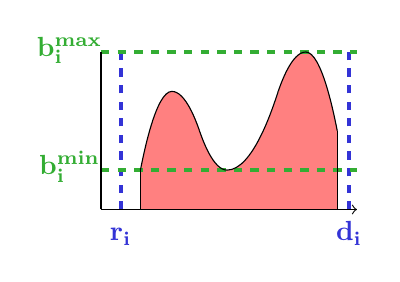
\begin{tikzpicture}
  [scale=0.5]
  \node (O) at (0,0) {};
  \fill[red!50] (1,0) -- (1,1) parabola bend (1.8,3)(2.51,2) -- (2.51,0);
  \fill[red!50] (2.49,0) -- (2.5,2) parabola bend (3.2,1) (4.511,3) -- (4.511,0) ;
  \fill[red!50] (4.489,0) -- (4.5,3) parabola bend (5.2,4) (6,2) -- (6,0);

  \node[label={[shift={(0,-0.7)}]\color{blue!80!black!80}$\mathbf{r_i}$}]  at (0.5,0) {};
  \node[label={[shift={(0,-0.7)}]\color{blue!80!black!80}$\mathbf{d_i}$}]  at (6.3,0) {};
  \draw[ultra thick,dashed,color=blue!80!black!80] (0.5,0) -- (0.5,4);
  \draw[ultra thick,dashed,color=blue!80!black!80] (6.3,0) -- (6.3,4);
  
    \node[label={[shift={(-0.4,-0.4)}]\color{green!60!black!80}$\mathbf{b_i^{min}}$}]  at (0,1) {};
    \node[label={[shift={(-0.4,-0.4)}]\color{green!60!black!80}$\mathbf{b_i^{max}}$}]  at (0,4) {};
    \draw[ultra thick,dashed,color=green!60!black!80] (0,1) -- (6.5,1);
    \draw[ultra thick,dashed,color=green!60!black!80] (0,4) -- (6.5,4);
  
  \draw (O.center) -- (0,4);
  \draw[->] (O.center) -- (6.5,0);
  
  \draw (1,1) -- (1,0);
  
  
  \draw (1,1) parabola bend (1.8,3)(2.5,2); 
  \draw (2.5,2) parabola bend (3.2,1) (4.5,3);
  \draw (4.5,3) parabola bend (5.2,4) (6,2);
  
  \draw (6,2) -- (6,0);
\end{tikzpicture}

         \end{column}
         \begin{column}{0.45\linewidth}
           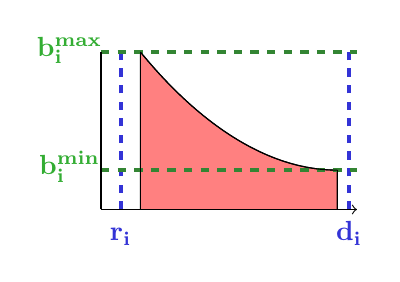
\begin{tikzpicture}
  [scale=0.5]
  \node (O) at (0,0) {};
    \path[draw, fill=red!50] (1,0) -- (1,4) parabola [bend at end] (6,1) -- (6,0); 
  
    \node[label={[shift={(0,-0.7)}] \color{blue!80!black!80}$\mathbf{r_i}$}]  at (0.5,0) {};
    \node[label={[shift={(0,-0.7)}] \color{blue!80!black!80}$\mathbf{d_i}$}]  at (6.3,0) {};
    \draw[ultra thick,dashed,color=blue!80!black!80] (0.5,0) -- (0.5,4);
    \draw[ultra thick,dashed,color=blue!80!black!80] (6.3,0) -- (6.3,4);

    \node[label={[shift={(-0.4,-0.4)}] \color{green!60!black!80}$\mathbf{b_i^{min}}$}]  at (0,1) {};
    \node[label={[shift={(-0.4,-0.4)}] \color{green!60!black!80}$\mathbf{b_i^{max}}$}]  at (0,4) {};
    \draw[ultra thick,dashed,color=green!40!black!80] (0,1) -- (6.5,1);
    \draw[ultra thick,dashed,color=green!40!black!80] (0,4) -- (6.5,4);
  
  
  \draw (O.center) -- (0,4);
  \draw[->] (O.center) -- (6.5,0);
  
  \draw (1,4) -- (1,0);
  
  
  \path[draw] (1,4) parabola [bend at end] (6,1); 
  
  \draw (6,1) -- (6,0);
\end{tikzpicture}

         \end{column}
       \end{columns}
       \vfill}
     \only<8>{
       \vfill
       \begin{itemize}
       \item Modeled with a continuous resource
       \end{itemize}
       \vfill 
       $\Rightarrow$ \textbf{Continuous Energy-Constrained Scheduling Problem (CECSP) {\scriptsize \color{gray!50!black!50} \it [Artigues \& Lopez, JoS, 2015]}}
       \vfill}
   \end{overlayarea}
 \end{frame}
 
 \begin{frame}
   \frametitle{Problem statements}
   \vfill
   Input:\\
   \begin{itemize}
   \item $A=\{1,\hdots,n\}$ a set of non-preemptive tasks
   \item a continuous, cumulative and renewable resource of capacity  $B$
   \end{itemize}
   \vfill
   \onslide<2->{
     Output: A scheduling, i.e. a start time $st_i$, an end time $ft_i$ and a resource allocation function $b_i(t)$, such that:
   }
   \begin{overlayarea}{\linewidth}{1cm}
     \only<3>{\[est_i\le st_i\le ft_i \le lst_i\]}
     \only<4>{\[\bmin \le b_i(t) \le \bmax \quad \forall t \in \inter[st_i][ft_i]\]}
     \only<5>{\[b_i(t)=0\quad \forall t \not\in \inter[st_i][ft_i]\]}
     \only<6>{\[\int_{st_i}^{ft_i}b_i(t)dt=W_i\]}
     \only<7>{\[\sum_{i\in A}b_i(t) \le B\]} 
   \end{overlayarea}
   \onslide<2->{
     \begin{center}
       \begin{tikzpicture}
  [yscale=0.5,xscale=1]
  \node[] (O) at (0,0) {};
  
  \onslide<6>
      {
        \fill[red!50] (1,0) -- (1,3) -- (6,2) -- (6,0);
        \node[fill=red!50] at (3.5,1.5) {\textcolor{red}{$\int b_i(t) dt$}};
      }

      \onslide<3->
          {
            \node[label={[shift={(0,-0.7)}]\color{gray!30!}\color<3>{red}$r_i$}]  at (0.5,0) {};
            \node[label={[shift={(0,-0.7)}]\color{gray!30!}\color<3>{red}$d_i$}]  at (6.6,0) {};
                 {\color{gray!30!}
                   \color<3>{red}
                   \draw[dashed] (0.5,0) -- (0.5,4);
                   \draw[dashed] (6.6,0) -- (6.6,4);
          }}
          \onslide<4->{
            \node[label={[shift={(-0.4,-0.4)}]\color{gray!30!}\color<4>{red}$b_i^{min}$}]  at (0,0.9) {};
            \node[label={[shift={(-0.4,-0.4)}]\color{gray!30!}\color<4>{red}$b_i^{max}$}]  at (0,3) {};
                 {\color{gray!30!}
                   \color<4>{red}
                   \draw[dashed] (0,0.9) -- (6.5,0.9);
                   \draw[dashed] (0,3) -- (6.5,3);
          }}
          \draw[dashed,gray!30!] (0,3.7) -- (7,3.7) node [right] {$B$};
          \only<7>{
            \draw[dashed,red] (0,3.7) -- (7,3.7) node [right] {$B$};
          }
          \draw[->] (O.center) -- (0,4.3) node[left] {$b_i(t)$};
          \draw[->] (O.center) -- (7.5,0) node[below] {$t$};

          \draw (1,3) -- (1,0) node[below] {$st_i$};
          \draw (1,3) -- (6,2);
          \draw (6,2) -- (6,0) node[below] {$et_i$};


          \only<5>{
            \draw[red,thick] (0,0) -- (1,0);
            \draw[red,thick] (6,0) -- (7.5,0);
          }
\end{tikzpicture}

     \end{center}}
 \end{frame}
 
 \begin{frame}
  \frametitle{Example}
  \begin{center}
    \begin{tabular}{cccccc}
      \hline
      $i$ & $r_i$ & $d_i$ & $W_i$ & $b_i^{min}$ & $b_i^{max}$ \\
      \hline
      {\color<3-4>{red!80!black!80}$1$} &
                                          {\color<3-4>{red!80!black!80}$0$} & {\color<3-4>{red!80!black!80}$6$} & {\color<3-4>{red!80!black!80} $12$} & {\color<3-4>{red!80!black!80} $1$ }& {\color<3-4>{red!80!black!80} $5$} \\
      $2$ & $2$ & $6$ & $12$ & $2$ & $5$ \\
      $3$ & $2$ & $5$ & $6$ & $2$ & $2$ \\
      \hline
    \end{tabular}
  \end{center}
  
  \pause
  \begin{columns}
    \begin{column}{0.45\linewidth}
      \onslide<2->{
        \begin{tikzpicture}
[scale=0.7]
\node (O) at (0,0) {};
\node[label={[shift={(-0.4,0)}]$B=5$}] (B) at (0,5) {};

\onslide<3->{
\node[label={[shift={(-0.4,-0.4)}]\color{red!80!black!80}$b_1^{min}$}] (B) at (0,1) {};
\node[label={[shift={(-0.4,-0.4)}]\color{red!80!black!80}$b_1^{max}$}] (B) at (0,5) {};
}

\node (r1) at (0,-0.5) {{\color<3->{red!80!black!80}$est_1$}}; 
\node (r2) at (2,-0.5) {$est_2$};
\node (r3) at (2,-0.9) {$est_3$};
\node (d1) at (6,-0.5) {{\color<3->{red!80!black!80}$let_1$}};
\node (d2) at (6,-0.9) {$let_2$};
\node (d3) at (5,-0.5) {$let_3$};


\draw[->,>=latex] (6,0) -- (6.5,0);

%\draw (0,0) rectangle (6,5);
\draw[fill=blue!80!black!80] (4,0) -- (6,0) -- (6,5) -- (5,5) -- (5,3) -- (2,3) -- (2,1) --
(4,1) --cycle;
\onslide<2-3>
    {\draw[fill=red!80!black!80] (2,5) -- (2,1) -- (4,1) -- (4,0) -- (0,0) -- (0,5) -- cycle;}
\onslide<3->
    {\draw[fill=red!80!black!80] (2,5) -- (2,1) -- (4,1) -- (4,0) -- (0,0) -- (0,5) -- cycle;}
% \onslide<7>
%     {\draw[fill=red!80!black!80] (2,5) -- (2,0) -- (0,0) -- (0,5)-- cycle;
%       \draw[fill=red!80!black!80,pattern=north west lines, pattern color=red!80!black!80] (2,1) -- (4,1) -- (4,0)-- (2,0) -- cycle;
%     }
% \onslide<8->
%     {\draw[fill=red!80!black!80,pattern=north west lines, pattern color=red!80!black!80] (2,1) -- (4,1) -- (4,0)-- (0,0) --(0,5)--(2,5) -- cycle;
%     }
\draw[fill=orange!80!black!80]  (2,3) -- (5,3) -- (5,5) -- (2,5) --cycle;


\node (2) at (4,2) {\LARGE $2$};
\node (1) at (1,2) {\LARGE $1$};
\node (3) at (3.5,4) {\LARGE $3$};
\foreach \i in {0,...,5}
{
  \draw (\i,-0.3) -- (\i,0);
  \draw (-0.3,\i) -- (0,\i);
}

 \draw (6,-0.3) -- (6,0);

\end{tikzpicture}

      }
    \end{column}
    \hfill
    \begin{column}{0.45\linewidth}
      \newbox\hautbox \setbox\hautbox=\hbox{\vphantom{\rule[-0.4cm]{0cm}{0.9cm}}}
      \begin{tabular}{@{\usebox{\hautbox}}l}
        \onslide<4->{$\int_0^{4} b_1(t)dt=?$} \\
        \onslide<5->{$\int_0^{2}${\color<5>{red!80!black!80}{$5$}}$dt$}\onslide<6->{$+\int_2^{4}${\color<6>{red!80!black!80}{$1$}}$dt$}\\
        \onslide<7->$=10+2=12$\\
      \end{tabular}
    \end{column}
    \hfill
  \end{columns}
\end{frame}

 
 \begin{frame}{The CECSP : limitations}
   \vfill
   \begin{itemize}
   \item Consider that the resource consumed by the task is proportional to
     the energy received by the task.
     \vfill
     \pause
   \item Not always the case...
   \end{itemize}
   \vfill
   \pause
   \begin{block}{Example in parallel architecture}
     \begin{itemize}
     \item a set of tasks has to be scheduled on parallel processors;
       \pause
     \item resource : processors;
       \pause
     \item energy : elementary operation;
       \pause
     \item Typical power speed function:  $b^{\alpha} , \ 0 <
       \alpha \le 1$ (may be different for each task)
       \pause
     \end{itemize}
   \end{block}
   \vfill

 \end{frame}
 
 \begin{frame}{The CECSP : limitations}
   \begin{itemize}
   \item   $\Rightarrow$ We need to model conversion functions $f_i$.
     \vfill
\pause
   \item  We have considered the case where $f_i(b)$ is non-decreasing,
     continuous and  
\pause
     \begin{enumerate}
     \vspace{0.5cm}
     \item linear: $f_i(b)=a_i*b+c_i$ 

     \vspace{0.1cm}
       $\rightarrow$ the {\bf CECSP$_{lin}$}
     \vspace{0.5cm}
\pause
     \item concave and piecewise linear: if $f$ has $P$ pieces,
       $f_i(b)=a_{ip}*b+c_{ip}  , p \in \{1,\dots,P\}$

     \vspace{0.1cm}
       $\rightarrow$ {\bf the CECSP$_{cpwl}$} 
     \end{enumerate}
     \vfill
\pause
   \item   \[W_i=\int_{st_i}^{ft_i}b_i(t)dt \rightarrow W_i=\int_{st_i}^{ft_i}f_i(b_i(t))dt\]
     \vfill
\pause
   \item   linear and concave piecewise linear approximation of more
     general efficiency functions.
 \end{itemize}
   \vfill
 \end{frame}
 
\begin{frame}
  \frametitle{Concave Efficiency Function}
  $f_i$ are continuous, non-decreasing and {\bf concave} efficiency functions 
  \vfill
  \begin{columns}
    \begin{column}{0.45\linewidth}
      \begin{figure}
        \centering
        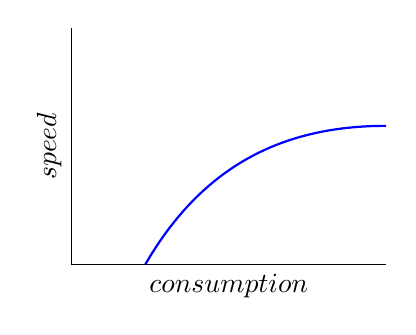
\begin{tikzpicture}
          \node (O) at (0,0) {};
          \draw (0,0) -- (4,0) node[midway,below] {$consumption$};
          \draw (0,0) -- (0,3) node[midway,left] {\rotatebox{90}{$speed$}};
          \draw[thick,blue] (0.94,0) to [bend left] (4,1.76);
        \end{tikzpicture}
        \caption{Speed vs. fuel consumption\footnotemark}
      \end{figure}
    \end{column}
    \hfill
    \begin{column}{0.45\linewidth}      
      \vspace{0.2cm}
      \begin{figure}
        \centering    
        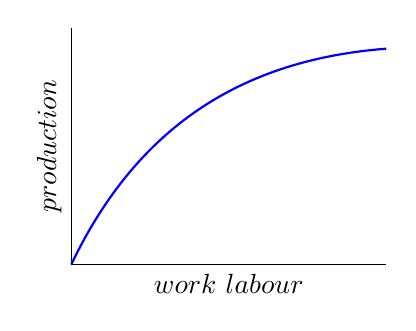
\begin{tikzpicture}
          \node (O) at (0,0) {};
          \draw (0,0) -- (4,0) node[midway,below] {$work\ labour$};
          \draw (0,0) -- (0,3) node[midway,left] {\rotatebox{90}{$production$}};
          \draw[thick,blue] (0,0) to [bend left] (4,2.74);
        \end{tikzpicture}      
        \caption[\footnotesize]{ Work Labour vs. production rate\footnotemark}
      \end{figure}
    \end{column}
    \hfill
  \end{columns}
  \footnotetext[1]{\tiny Algebra Symposium: Optimizing Fuel Consumption}
  \footnotetext[2]{\tiny Non-convex agreggative technology
    and optimal economic growth}
\end{frame}


 \begin{frame}{Approximation of efficiency functions with the CECSP$_{lin}$}
   \begin{block}{}
     \begin{tabularx}{\textwidth}{XXX}
       $b_i^{min}=0.25$&
       $b_i^{max}=1$&
       $f_i(b)=\sqrt{b}$
     \end{tabularx} 
   \end{block}
 \vfill
\pause
  \begin{columns}
     \begin{column}{0.5\linewidth}
       \begin{figure}[!htb]
         \centering
         \begin{tikzpicture}
           [xscale=3,yscale=2.5]
           \node (O) at (0,0) {};

           \draw[->] (0,0) -- (1.28,0) node[below] {\footnotesize $b$};
           \draw[->] (0,0) -- (0,1.3) node[left] {\footnotesize $f_i(b)$};

           \draw (0,1) -- (-0.02,1) node[left] {\footnotesize $1$};
           \draw (0,0.5) -- (-0.02,0.5) node[left] {\footnotesize $\sqrt{0.25}$};

           \draw (1,0) -- (1,-0.02) node[below] {\footnotesize $1$};
           \draw (0.25,0) -- (0.25,-0.02) node[below] {\footnotesize $0.25$};

           \draw[color=gray,domain=0:1.28,samples=50] plot ({\x},{sqrt(\x)});
           \draw[dashed,thick,domain=0.25:1,samples=50] plot
           ({\x},{\x/(2*sqrt(0.625))+sqrt(0.625)/2});


           \draw[dotted] (0.25,0)-- (0.25,1.3);
           \draw[dotted] (1,0) -- (1,1.3);
         \end{tikzpicture}
         \caption{Approximation by a linear function}
       \end{figure}
     \end{column}
\pause
     \hfill
     \begin{column}{0.5\linewidth}
       \begin{figure}[!htb]
         \centering
         \begin{tikzpicture}
           [xscale=3,yscale=2.5]
           \node (O) at (0,0) {};

           \draw[->] (0,0) -- (1.28,0) node[below] {\footnotesize $b$};
           \draw[->] (0,0) -- (0,1.3) node[left] {\footnotesize $f_i(b)$};

           \draw (0,1) -- (-0.02,1) node[left] {\footnotesize $1$};
           \draw (0,0.5) -- (-0.02,0.5) node[left] {\footnotesize $\sqrt{0.25}$};

           \draw (1,0) -- (1,-0.02) node[below] {\footnotesize $1$};
           \draw (0.25,0) -- (0.25,-0.02) node[below] {\footnotesize $0.25$};

           \draw[color=gray,domain=0:1.28,samples=50] plot ({\x},{sqrt(\x)});
           
           \draw[ dashed,thick,domain=0.25:0.5,samples=50] plot
           ({\x},{\x/(2*sqrt(0.375))+sqrt(0.375)/2});
           \draw[dashed, thick,domain=0.5:0.75,samples=50] plot
           ({\x},{\x/(2*sqrt(0.625))+sqrt(0.625)/2});
           \draw[dashed, thick,domain=0.75:1,samples=50] plot
           ({\x},{\x/(2*sqrt(0.875))+sqrt(0.875)/2});

           \draw[dotted] (0.5,0)-- (0.5,1.3);
           \draw[dotted] (0.25,0) -- (0.25,1.3);
           \draw[dotted] (0.75,0) -- (0.75,1.3);
           \draw[dotted] (1,0) -- (1,1.3);
         \end{tikzpicture}
         \caption{Approximation by a concave piecewise linear function}
       \end{figure}
     \end{column}
   \end{columns}

 \end{frame}

 \begin{frame}{Example for the CECSP$_{lin}$}
   

\begin{columns}
  \begin{column}{0.5\linewidth}
    \begin{center}
      {\small \begin{tabular}{|M{0.4cm}|M{0.4cm}M{0.4cm}M{0.4cm}M{0.4cm}M{0.4cm}M{1.2cm}|}
        \hline
        $i$ & $r_i$ & $d_i$ & $W_i$ & $\bmin$ & $\bmax$ & $f_i(b)$\\[1mm]
        \hline
        1 & 0 & 2 & 6 & 3 & 3 & $b$\\[1mm]
        \color<3->{red!80!black!80}2 & \color<3->{red!80!black!80}1 & \color<3->{red!80!black!80}5 & \color<3->{red!80!black!80}22 & \color<3->{red!80!black!80}3 & \color<3->{red!80!black!80}4 & \color<3->{red!80!black!80}$\rightarrow$ \\[1mm]
         3 & 0 &6 & 45 & 1 & 5 & $3b+1$\\[1mm]
        \hline
        \multicolumn{7}{c}{}
      \end{tabular}}
    \end{center}
  \end{column}
\hfill
    \begin{column}{0.4\linewidth}
\begin{tikzpicture}
[xscale=0.8,yscale=0.45]
\node (O) at (2,5) {};
\draw[->] (2,4) -- (5.5,4) node[below] {$b$}; 
\draw[dashed] (2,4) -- (2,5.5);
\draw[->] (2,5.5) -- (2,10) node[left] {$f_2(b)$};


\path[draw] (3,6) -- (4,8) -- (5,9) ;

\draw[dotted] (3,4) node[below] {\footnotesize $3$} -- (3,10);
\draw[dotted,color=gray!70] (4,4) node[below,color=black] {\footnotesize $4$}
-- (4,10);
\draw[dotted] (5,4) node[below] {\footnotesize $5$} -- (5,10);

\draw (2,6) node[left] {\footnotesize $6$};
\draw (2,8) node[left] {\footnotesize $8$};
\draw (2,9) node[left] {\footnotesize $9$};
\end{tikzpicture}
\end{column}
\end{columns}
\pause
  \begin{columns}
    \begin{column}{0.45\linewidth}
      \onslide<2->{
        \centering
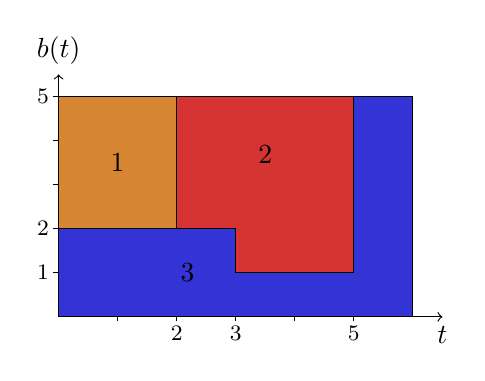
\begin{tikzpicture}
[xscale=0.75,yscale=0.56]
\node (O) at (0,0) {};
\draw[->] (0,0) -- (6.5,0) node[below] {$t$};
\draw[->] (0,0) -- (0,5.5) node[above] {$b(t)$};

\draw[fill=orange!80!black!80] (0,2) rectangle (2,5) node[midway] {$1$};
\path[draw,fill=blue!80!black!80] (0,0) -- (0,2) -- (3,2) -- (3,1) node[left=0.4cm] {$3$} -- (5,1) -- (5,5) -- (6,5)  -- (6,0) -- cycle;
\draw[fill=red!80!black!80] (2,5) -- (5,5) node[midway,below=0.5cm] {$2$} -- (5,1) -- (3,1) -- (3,2) -- (2,2) -- cycle;

\draw (0,1) node[left] {\footnotesize $1$};
\draw (0,2) node[left] {\footnotesize $2$};
\draw (0,5) node[left] {\footnotesize $5$};


\draw (2,0) node[below] {\footnotesize $2$};
\draw (3,0) node[below] {\footnotesize $3$};
\draw (5,0) node[below] {\footnotesize $5$};

\foreach \i in {1,...,5}{
\draw (\i,-0.1) -- (\i,0);
\draw (-0.1,\i) -- (0,\i);
}
\end{tikzpicture}

      }
    \end{column}
    \hfill
       \begin{column}{0.45\linewidth}{
\vspace{-0.1cm}       
       \small
      \newbox\hautbox \setbox\hautbox\hbox{\vphantom{\rule[-0.4cm]{0cm}{0.8cm}}}
      \begin{tabular}{@{\usebox{\hautbox}}l}
        \onslide<4->{$\int_2^{5} f_2(b_2(t))dt=?$} \\
        \onslide<5->{$\int_2^{3} f_2(3) dt$}\onslide<6->{$+\int_3^{5} f_2(4) dt$=}\\
	    \onslide<7->{$\int_2^{3} 6 dt$}\onslide<8->{$+\int_3^{5} 8 dt$=}\\
       \onslide<9->{$6$}\onslide<10->{$+16=$}\onslide<11->{$22$}\\
              \end{tabular}}
    \end{column}
    \hfill
  \end{columns}

 \end{frame}

 \begin{frame}
   \frametitle{Solution methods}
   \vfill
   \begin{description}[Properties]
   \item[Properties] {\small
       \begin{itemize}
       \item study of the structural properties of the problem:
         {\footnotesize Dominance rules, complexity analysis, polynomial cases...}
       \end{itemize}}
     \vfill
\pause
   \item[CP] {\small
       \begin{itemize}
       \item satisfiability test (checker): {\footnotesize Energetic
           reasoning, Flow based checker...}
       \item filtering algorithm: {\footnotesize Energetic reasoning, time-table
           disjunctive reasoning...}
       \item discrete model
       \end{itemize}}
     \vfill
\pause
   \item[MILP] {\small
       \begin{itemize}
       \item MILP model: {\footnotesize time-indexed, event-based...}
       \item valid inequalities
       \item polyhedral results
       \end{itemize}}
     \vfill
\pause
   \item[Hybrid] {\small
       \begin{itemize}
       \item ``CP-like branching'' + MILP 
       \item valid inequalities deduced from ER
       \end{itemize}}
   \end{description}
 \end{frame}

 \setcounter{tocdepth}{20}
 \begin{frame}{Overview}
   \tableofcontents[hideothersubsections,subsubsectionstyle={show/show/show/show}]
 \end{frame}


% \setcounter{tocdepth}{1}
% \begin{frame}
%   \tableofcontents
% \end{frame}
% \addtocounter{framenumber}{-1}

\setcounter{tocdepth}{2}
\AtBeginSection[]
{
  \begin{frame}
    \frametitle{Overview}
    \tableofcontents[sectionstyle=show/shaded,subsectionstyle=show/show/hide
    ] 
  \end{frame}
  \addtocounter{framenumber}{-1}
}
\setcounter{tocdepth}{2}
\AtBeginSubsection[]
{
  \begin{frame}
    \frametitle{Overview}
    \tableofcontents[sectionstyle=show/shaded,subsectionstyle=show/shaded/hide ]
  \end{frame}
  \addtocounter{framenumber}{-1}
}
\section{Problem Properties}
\subsection{Simple Properties}
\begin{frame}
  \frametitle{Simple Properties}
  \begin{itemize}
\vfill
  \item NP-complete (CuSP is a particular case of CECSP)
\vfill
\pause
  \item scheduling a task at $\bmax$ during $\inter$ gives the higher energy amount ($f_i$ is non decreasing)
\vfill\end{itemize}
\begin{center}
    \begin{tikzpicture}
      [yscale=0.6]
      [inner sep=0]
      \node (O) at (0,0) {};
      \node (T) [right of=O,node distance=4cm] {};
      \node (t1) [right of =O, node distance=1cm] {};
      \node (t2) [right of =t1, node distance=2cm] {};
      \draw[pattern=north west lines] (t1) rectangle (3,2.5);
      \draw[dashed,gray!40!black!40] (0,2.5) -- (4,2.5) node[right] {$\bmax$};
      
      \draw[red,dashed] (t1) node[below] {$t_1$}-- (1,3);
      \draw[red,dashed] (t2) node[below] {$t_2$} -- (3,3);
      \draw[->] (O) -- (T);
    \end{tikzpicture}
  \end{center}

\pause

\vfill
  \begin{block}{Notations}
    \begin{itemize}
    \item the latest start time of $i$ as $lst_i=let_i-\frac{W_i}{f_i(\bmax)}$
    \item and the earliest end time of $i$ as $eet_i=est_i+\frac{W_i}{f_i(\bmax)}$
    \end{itemize}
  \end{block}
\vfill
\pause

  $\Rightarrow$ a task can start in $\inter[est_i][lst_i]$ and end in $\inter[eet_i][let_i]$
\vfill
\end{frame}
\subsection{Non-integer solution}
\begin{frame}
  \frametitle{Non-integer solution}
  \vfill
  \begin{itemize}
  \item   Instances with integer data can have only non-integer solution.
  \end{itemize}
  \vfill
\pause

  \begin{center}
    \begin{tabularx}{10cm}{|>{\centering\arraybackslash}p{0.6cm}|
        *5{>{\centering\arraybackslash}X}>{\centering\arraybackslash}p{2cm}|}
      \hline
      $i$ & $est_i$ & $lst_i$ & $W_i$ & $\bmin$ & $\bmax$ & $f_i(b_i(t))$ \\
      \hline
      $1$ & $0$ & $2$ & $18$ & $2$ & $2$ & $3b_i(t)+6$\\
      $2$ & $1$ & $3$ & $3$ & $1$ & $2$ & $b_i(t)$\\
      \hline
    \end{tabularx}
  \end{center}
  \vfill
\pause

  \centering
  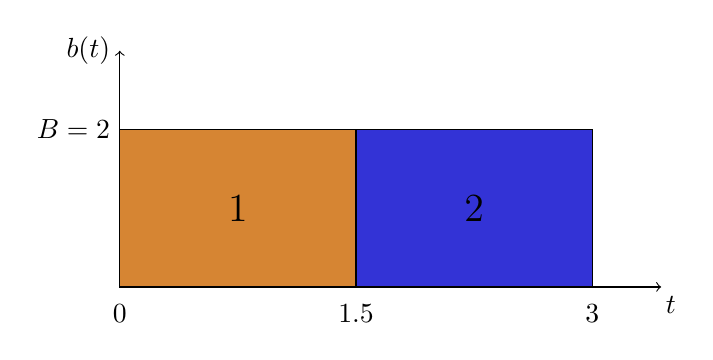
\begin{tikzpicture}
    [xscale=2]
    \node (O) at (0,0) {} node[below=0.1cm] {$0$};
    \draw (1.5,0)  node[below=0.1cm] {$1.5$};
    \draw (3,0) node[below=0.1cm] {$3$};
    \node (T) at (3.5,0) {};
    \draw(0,2)  node[left,node
    distance=1.5pt] {$B=2$}; 
    \draw[fill=orange!80!black!80] (O) rectangle (1.5,2);
    \draw[fill=blue!80!black!80] (1.5,2) rectangle (3,0);
    \draw[->] (0,0) -- (T) node[below] {$t$};
    \draw[->] (0,0) -- (0,3) node[left] {$b(t)$};
    
    \node at (0.75,1) {\Large 1};
    \node at (2.25,1) {\Large 2};
  \end{tikzpicture}
  \vfill  
\end{frame}

\subsection{Piecewise Constant Resource Allocation}
\begin{frame}{Piecewise Constant Resource Allocation}
  \begin{theorem}
    Any solution of \only<1-8>{\textcolor{blue!80!black!80}{CECSP$_{lin}$}}
    \only<9->{\textcolor{red!80!black!80}{CECSP$_{cpwl}$}} and can be transformed in a solution
    where $\forall i \in A,\ b_i(t)$ is piecewise constant.  
  \end{theorem}
  \onslide<2->{
    \begin{proof}[Proof (Sketch)]
      \begin{columns}
        \begin{column}{0.55\linewidth}
          \begin{itemize}
          \item<3-> $(t_q)$: series of start and end times
            \vspace{0.2cm}
          \item<4-> in $\inter[t_q][t_{q+1}]$, $b'_i(t)$ is set to the mean value of $b_i(t)$ over this interval
          \end{itemize}
          \begin{overlayarea}{\textwidth}{0.5cm}
            \only<8>{	
              \begin{itemize}
              \item same resource and {\color{blue!80!black!80}same} energy
              \end{itemize}
            }
            \only<9>{ \begin{itemize}
              \item same resource and {\color{red!80!black!80}more} energy\footnote{Jensen,
                  Sur les fonctions convexes et les in{\'e}galit{\'e}s entre les
                  valeurs moyennes, 1906.}
              \end{itemize}}
            \only<10->{\begin{itemize}
              \item $ft_i=$ value for which required energy is received        
              \end{itemize}}
          \end{overlayarea}
        \end{column}
        \begin{column}{0.45\linewidth}
          \onslide<2->{
            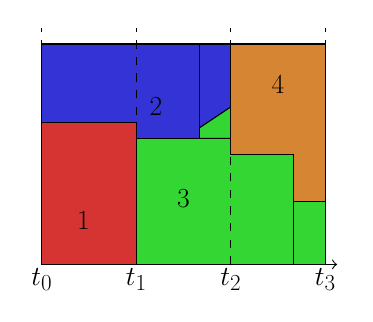
\begin{tikzpicture}
              [scale=0.4,transform shape]
              [inner sep =0]
              \node (O) at (0,0) {};
              \node (T) [right of=O,node distance=9.5cm] {};
              \onslide<2-9>{
                \fill[blue!80!black!80,draw=black] (0,3) rectangle (6,7) node[midway, right=0.8cm] { \color{black} \Huge $2$};}
              \onslide<2-4>{
                \fill[red!80!black!80,draw=black] (0,0) node[above right=1cm] { \color{black} \Huge $1$}-- (0,4) parabola bend (1.5,5) (3,4) --(3,0) -- cycle;}
              \onslide<5-9>{
                \fill[red!80!black!80,draw=black] (0,0) node[above right=1cm] {\color{black} \Huge $1$}-- (0,4.5) --(3,4.5) --(3,0) -- cycle;}
              \onslide<2-9>{
                \fill[orange!80!black!80,draw=black] (9,7) rectangle (6,2) node[midway, above= 0.8cm] {\color{black} \Huge $4$};}
              \onslide<2-5>{
                \fill[green!80!black!80,draw=black] (3,0) -- (9,0) -- (9,2) -- (6,5)-- (3,3)  node[below, right=2cm] { \color{black} \Huge $3$}-- cycle;}
              \onslide<6>{
                \fill[green!80!black!80,draw=black] (3,0) -- (9,0) -- (9,2) -- (6,5)-- (6,4)  node[left=1.5cm,below=1.5cm] { \color{black} \Huge $3$} --(3,4) -- cycle;
                ;}
              \onslide<7-9>{
                \fill[green!80!black!80,draw=black] (3,0) -- (9,0) -- (9,3.5) -- (6,3.5)-- (6,4)  node[left=1.5cm,below=1.5cm] { \color{black} \Huge $3$} --(3,4) -- cycle;
              }
              \draw[->] (O) -- (T);
              \onslide<10->{
                \fill[blue!80!black!80,draw=black] (0,3) rectangle (5,7) node[midway, right=0.8cm] { \color{black} \Huge $2$};
                \fill[red!80!black!80,draw=black] (0,0) node[above right=1cm] {\color{black} \Huge $1$}-- (0,4.5) --(3,4.5) --(3,0) -- cycle;
                \fill[orange!80!black!80,draw=black] (9,7) rectangle (6,2) node[midway, above= 0.8cm] {\color{black} \Huge $4$};
                \fill[green!80!black!80,draw=black] (3,0) -- (8,0) -- (8,3.5) -- (6,3.5)-- (6,4)  node[left=1.5cm,below=1.5cm] { \color{black} \Huge $3$} --(3,4) -- cycle;
              }       
              \onslide<3->{
                \draw[dashed] (0,0) node[below] {\color{black} \Huge $t_0$} -- (0,7.5);
                \draw[dashed] (3,0) node[below] {\color{black} \Huge $t_1$} -- (3,7.5);
                \draw[dashed] (6,0) node[below] {\color{black} \Huge $t_2$} -- (6,7.5);
                \draw[dashed] (9,0) node[below] {\color{black} \Huge $t_3$} -- (9,7.5);
              }


            \end{tikzpicture}
          }
        \end{column}
      \end{columns}
      \vspace{0.5cm}	
    \end{proof}}
\end{frame}
\subsection{Polynomial cases}
\begin{frame}{Polynomial cases}
  \vfill
  \begin{theorem}
    The CECSP, the CECSP$_{lin}$ and the CECSP$_{cpwl}$ with fixed
    task start and end times are polynomial.  
  \end{theorem}
  \vfill
\pause
 {\bf Proof (Sketch). } Only need to decide the quantity of resource
 given to tasks in each interval $[t_{q},t_{q+1}]$.


\pause
 Can be solved by a Flow-based Linear Program.
 \vfill
\pause
  \begin{theorem}
The preemptive CECSP, the preemptive CECSP$_{lin}$ and the preemptive CECSP$_{cpwl}$ are polynomial.  
  \end{theorem}
  \vfill
\pause
  
 {\bf Proof (Sketch). } Apply the Flow-based LP with $st_i=est_i$ and $ft_i=let_i$.
 \vfill
\end{frame}


% \begin{frame}{counter example concave function}
%   \vfill
%     \begin{theorem}
%     Any solution of CECSP$_{cpwl}$ and can be transformed in a
%     solution where $\forall i \in A,\ b_i(t)$ is piecewise constant. 
%   \end{theorem}
%   \vfill
%   Does not apply to the case of concave efficiency function.
%   \vfill
%   {\centering
%     \begin{tikzpicture}
% \node (O) at 
%     \end{tikzpicture}
%     }
%   \vfill 
% \end{frame}


\section{Hybrid Branch-and-Bound}
\subsection{Branching scheme}

\begin{frame}
  \frametitle{Branching scheme }
  \begin{itemize}
    \vfill
  \item Step 1: ER checker and ER adjustments on current node 
    \begin{itemize}
    \item If checker fails: backtrack
    \item else : go to Step 2
    \end{itemize}
    \vfill    
    \pause
  \item Step 2: Choose $st_i$ or $ft_i$ s.t. $[est_i,lst_i]$ or
    $[eet_i,let_i]$ min
    \vfill
    \pause
  \item Step 3: Create 2 nodes by separating the corresponding
    interval in 2 parts  {\small \it \color{gray!50!black!50} [Carlier
      \& Latapie, 1991]} 
  \end{itemize}
  \begin{overlayarea}{\textwidth}{4cm}
    \only<4>{
      \vfill
      {\it Ex with $st_i$:}
      \begin{center}
        \input{/home/mnattaf/Documents/input_latex/branching.tex}
      \end{center}
    }
    \only<5->{
      \begin{itemize}
      \item Repeat Steps 1--3 until each interval $\inter[est_i][lst_i]$ and $\inter[eet_i][let_i]$ has a size smaller than a given $\epsilon$ (DFS)\\
        \vspace{0.4cm}
        \pause
      \item MILP of the restricted problem
        \begin{itemize}
        \item If MILP solved the problem: STOP
        \item else : backtrack
        \end{itemize}
      \end{itemize}
    }
  \end{overlayarea}
  \vfill
\end{frame}

\subsection{Filtering algorithms}

\begin{frame}
  \frametitle{Energetic reasoning checker}
  {\small adaptation of the energetic reasoning for CuSP
    {\color{gray!50!black!50} \it [Baptiste et al., 2001]}}

  \vspace{0.4cm}
  \pause
  The {\bf slack function} of interval $\inter$ is:
  \begin{gather}
    SL(t_1,t_2)={\color<3>{red!80!black!80}\text{ available space in
      }\inter}-{\color<3>{blue!80!black!80}\text{ total mandatory }} \nonumber\\ 
    {\color<3>{blue!80!black!80}\text{consumption in } \inter}\nonumber
  \end{gather}
  \begin{theorem}
    If there exists an interval on which the slack function is negative then there is no solution
  \end{theorem}
  \vfill
  \onslide<3>{
    \begin{center}
      \begin{tikzpicture}
        [transform shape,xscale=0.7,yscale=0.5]
        [inner sep=0pt]
        \node (O) at (0,0) {};
        \node[right of=O, node distance=6cm] (T) {};
        \node[right of=O, node distance=2cm] (t1) {};
        \node[right of=O, node distance=4cm] (t2) {};
        
        \draw[dashed] (0,4) node[left] {\Large$B$} -- (6,4);

        \draw[->] (O) -- (T);

        \draw[thick,red] (t1) -- (2,4.5);
        \draw[thick,red] (t2) -- (4,4.5);

        \draw[fill=blue!50!black!50] (t1) node[above=2cm,left=0.6cm] {\color{blue!80!black!80} \Large mandatory consumption} rectangle (4.5,4);
        \draw[pattern=north west lines, pattern color=red] (t1) rectangle (4,4) node[below=2cm,right=0.8cm] {\color{red} \Large available resource};
      \end{tikzpicture}
    \end{center}}
\end{frame}

\begin{frame}
  \frametitle{Energetic reasoning checker}
  \vfill
  We define the {\bf mandatory consumption} of $i$ in interval $\inter$ as 
  \[\bb=\min \int_{t_1}^{t_2} b_i(t) dt\]
  \vfill
  In order to compute this quantity we also define the {\bf minimum energy
    consumption} of $i$ in interval $\inter$ as:
  \[\wb=\min \int_{t_1}^{t_2} f_i(b_i(t)) dt\]
\end{frame}


\begin{frame}{Mandatory consumption possible configurations}
  \vfill
\begin{columns}[b]
  \begin{column}{0.45\linewidth}
    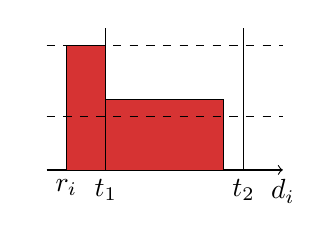
\begin{tikzpicture} [xscale=0.5,yscale=0.45]
      \node (O) at (0,0) {};
      \draw [->] (0,0) -- (6,0);
      \fill[red!80!black!80] (0.5,0) rectangle (1.5,3.5);
      \fill[red!80!black!80] (1.5,0) rectangle (4.5,2);
      \draw (0.5,0) node[below] {$r_i$};
      \draw (6,0) node[below] {$d_i$};
      \draw (1.5,0) node[below] {$t_1$} -- (1.5,4);
      \draw (5,0) node[below] {$t_2$} -- (5,4);
      \draw[dashed] (0,1.5) node[left] {$\bmin$} -- (6,1.5);
      \draw[dashed] (0,3.5) node[left] {$\bmax$} -- (6,3.5);
      \draw (0.5,0) -- (0.5,3.5) -- (1.5,3.5) -- (1.5,2) -- 
      (4.5,2) -- (4.5,0);
    \end{tikzpicture}
    \begin{center}
      {\small left-shifted}
    \end{center}
  \end{column}
\hfill  
\begin{column}{0.45\linewidth}  
  \onslide<2->{
      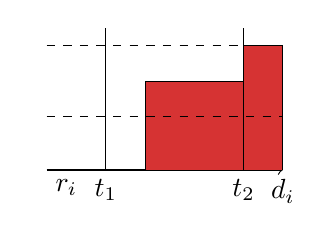
\begin{tikzpicture} [xscale=0.5,yscale=0.45]
        \node (O) at (0,0) {};
        \draw [->] (0,0) -- (6,0);
        \fill[red!80!black!80] (5,0) rectangle (6,3.5);
        \fill[red!80!black!80] (5,0) rectangle (2.5,2.5);
        \draw (0.5,0) node[below] {$r_i$};
        \draw (6,0) node[below] {$d_i$};
        \draw (1.5,0) node[below] {$t_1$} -- (1.5,4);
        \draw (5,0) node[below] {$t_2$} -- (5,4);
        \draw[dashed] (0,1.5) node[left] {$\bmin$} -- (6,1.5);
        \draw[dashed] (0,3.5) node[left] {$\bmax$} -- (6,3.5);
        \draw (6,0) -- (6,3.5) -- (5,3.5) -- (5,2.5) --
        (2.5,2.5) -- (2.5,0);
      \end{tikzpicture}        
      \begin{center}
        {\small right-shifted}
      \end{center}
    }
  \end{column}
\end{columns}
\vfill
\begin{columns}[b]
  \begin{column}{0.45\linewidth}
    \onslide<3->{
      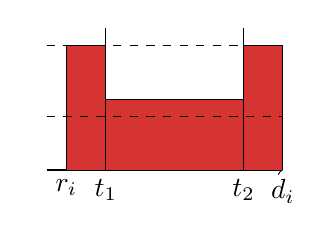
\begin{tikzpicture} [xscale=0.5,yscale=0.45]
        \node (O) at (0,0) {};
        \draw [->] (0,0) -- (6,0);
        \fill[red!80!black!80] (0.5,0) rectangle (1.5,3.5);
        \fill[red!80!black!80] (6,0) rectangle (5,3.5);
        \fill[red!80!black!80] (5,0) rectangle (1.5,2);
        \draw (0.5,0) node[below] {$r_i$};
        \draw (6,0) node[below] {$d_i$};
        \draw (1.5,0) node[below] {$t_1$} -- (1.5,4);
        \draw (5,0) node[below] {$t_2$} -- (5,4);
        \draw[dashed] (0,1.5) node[left] {$\bmin$} -- (6,1.5);
        \draw[dashed] (0,3.5) node[left] {$\bmax$} -- (6,3.5);
        \draw (0.5,0) -- (0.5,3.5) -- (1.5,3.5) -- (1.5,2) --
        (5,2) -- (5,3.5) -- (6,3.5) -- (6,0) ;
      \end{tikzpicture} 
      \begin{center}
      {\small both-shifted 1}
    \end{center}}
  \end{column}
  \hfill
\begin{column}{0.45\linewidth}
    \begin{overlayarea}{0.45\linewidth}{3.5cm}
      \only<4>{
        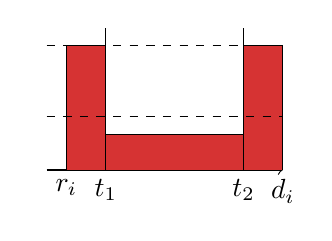
\begin{tikzpicture} [xscale=0.5,yscale=0.45]
          \node (O) at (0,0) {};
          \draw [->] (0,0) -- (6,0);
          \fill[red!80!black!80] (0.5,0) rectangle (1.5,3.5);
          \fill[red!80!black!80] (6,0) rectangle (5,3.5);
          \fill[red!80!black!80] (5,0) rectangle (1.5,1);
          \draw (0.5,0) node[below] {$r_i$};
          \draw (6,0) node[below] {$d_i$};
          \draw (1.5,0) node[below] {$t_1$} -- (1.5,4);
          \draw (5,0) node[below] {$t_2$} -- (5,4);
          \draw[dashed] (0,1.5) node[left] {$\bmin$} -- (6,1.5);
          \draw[dashed] (0,3.5) node[left] {$\bmax$} -- (6,3.5);
          \draw (0.5,0) -- (0.5,3.5) -- (1.5,3.5) -- (1.5,1) --
          (5,1) -- (5,3.5) -- (6,3.5) -- (6,0) ;
        \end{tikzpicture}
      }
      \only<5-> {
        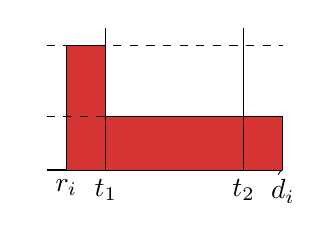
\begin{tikzpicture} [xscale=0.5,yscale=0.45]
          \node (O) at (0,0) {};
          \draw [->] (0,0) -- (6,0);
          \fill[red!80!black!80] (0.5,0) rectangle (1.5,3.5);
          \fill[red!80!black!80] (6,0) rectangle (1.5,1.5);
          \draw (0.5,0) node[below] {$r_i$};
          \draw (6,0) node[below] {$d_i$};
          \draw (1.5,0) node[below] {$t_1$} -- (1.5,4);
          \draw (5,0) node[below] {$t_2$} -- (5,4);
          \draw[dashed] (0,1.5) node[left] {$\bmin$} -- (6,1.5);
          \draw[dashed] (0,3.5) node[left] {$\bmax$} -- (6,3.5);
          \draw (0.5,0) -- (0.5,3.5) -- (1.5,3.5) -- (1.5,1.5) --
          (6,1.5)  -- (6,0) ;
        \end{tikzpicture}
      }
      \onslide<4->{
      \begin{center}
        {\small both-shifted 2}
      \end{center}}
    \end{overlayarea}
  \end{column}
\end{columns}

  \onslide<6>{
    \[\wb = \min ( LS, RS, \max (BS_1,BS_2))\]
  }
\end{frame}

\begin{frame}
  \frametitle{Minimal resource consumption}
  \begin{center}
      \begin{tikzpicture}
  [yscale=0.5,xscale=0.7]
    \node[] (O) at (0,0) {};
    \node[label={[shift={(-0.4,-0.4)}]$b_i^{min}$}] (bmin) at (0,1) {};
    \node[label={[shift={(-0.4,-0.4)}]$b_i^{max}$}] (bmax) at (0,4) {};
    \node[label={[shift={(0,-0.8)}]$t_1$}] (t1) at (4,0) {};
    \node[label={[shift={(0,-0.8)}]$t_2$}] (t2) at (7,0) {};
    \node[label={[shift={(0,-0.8)}]$d_i$}] (di) at (6,0) {};
    \node[label={[shift={(0,-0.8)}]$r_i$}] (ri) at (1,0) {};
    
    \draw[->] (O.center) -- (8,0);
    \draw (O.south) -- (bmax.north);
    \draw (bmin.center) -- (8,1);
    \draw (bmax.center) -- (8,4);
    \draw[fill=white] (ri.center) rectangle (4,4);
    \draw[pattern=north west lines] (ri.center) rectangle (4,4);
    \draw[fill=white] (t1.center) rectangle (5,1.5);
    \draw[pattern=north west lines] (t1.center) rectangle (5,1.5);
    \draw(di.south) -- (di.center);
    \draw(ri.south) -- (ri.center);
    \draw[thick,color=green!80!black!80] (t1.south) -- (4,4.1);
    \draw[thick,color=green!80!black!80] (di.south) -- (6,4.1);
    \draw[] (t2.south) -- (7,4.1);

    \draw[color=green!80!black!80,thick,decorate,decoration={brace,raise=0.1cm}] (4,4) -- (6,4) node[above=0.2cm,pos=0.5] {J};

  \end{tikzpicture}

  \end{center}
  \vfill
  \pause
  \textbf{Question : }
  How can we bring an {\bf energy} $\mathbf{\wb}$ to $i$ in interval $J$ by consuming
  {\bf as few resource} as possible? 
  \vfill
  \pause
  \begin{align*}
    \text{ min }& \int_{J} b_i(t)dt  &\\
    \text{ s.t. } & \int_{J}f_i(b_i(t))dt \ge  \underline{w}(i,t_1,t_2)& \\
                &  \bmax \ge b_i(t) \ge \bmin \qquad \forall t \in J
  \end{align*}
  \vfill
\end{frame}

\begin{frame}
  \frametitle{Analytic expression of $\bb$}
  \vfill
  \begin{itemize}
  \item  \textbf{Question : }
    How can we bring an energy $\wb$ to $i$ in interval $J$ by consuming as few resource as possible?
    \vfill
    \begin{align*}
      \text{ min }& \int_{J} b_i(t)dt  \\
      \text{ s.t. } & \int_{J}f_i(b_i(t))dt \ge  \underline{w}(i,t_1,t_2) \\
                  &  \bmax \ge b_i(t) \ge \bmin\qquad \forall t \in J
    \end{align*}
    \vfill
  \item Theorem "piecewise constant $b_i(t)$" $\Rightarrow$ there is a constant $b_{i} > 0 $
    s.t. 
    \pause
    \begin{align*}
      \text{min }  & \int_{J} b_i\,dt  \\
      \text{s.t } & \int_{J}f_i(b_i)\,dt \ge
                    \underline{w}(i,t_1,t_2)\\
                   & \bmax \ge b_i \ge \bmin
    \end{align*}
  \end{itemize}
  \vfill
\end{frame}

\begin{frame}
  \frametitle{Analytic expression of $\bb$}
  \vfill
  $\bullet$ if $f_i$ is linear, i.e. of the form $f_i(b)= a_i*b+c_i$ :
  \pause
  \begin{align*}
    \text{min }  & \int_{J} b_i\,dt  \\
    \text{s.t } & \int_{J}(a_i*b_i+c_i)\,dt \ge
                  \underline{w}(i,t_1,t_2)\\
                 & \bmax \ge b_i \ge \bmin
  \end{align*}
  \pause
  { \color{blue!80!black!80}
    $\boldmath{\Rightarrow  \underline{b}(i,t_1,t_2)= \max ( |J|\bmin, \frac{1}{a_i}( \underline{w}(i,t_1,t_2)-|J|c_i))}$}.
  
\end{frame}

\begin{frame}
  \frametitle{Analytic expression of $\bb$}
  \vfill
  $\bullet$  if $f_i$ is concave and piecewise linear, i.e. of the form
  $f_i(b)=a_{ip}*b+c_{ip}, \forall p \in {\cal P}$:
  \pause

  \begin{align*}
    \text{min }  & \int_{J} b_i\,dt  \\
    \text{s.t } & \int_{J}(a_{ip}*b_i+c_{ip})\,dt \ge
                  \underline{w}(i,t_1,t_2) \qquad \forall p \in
                  {\cal P}\\
                 & \bmax \ge b_i \ge \bmin
  \end{align*}
  \pause
  { \color{blue!80!black!80}
    $\boldmath{\Rightarrow  \underline{b}(i,t_1,t_2)= \max ( |J|\bmin, \max_{p
        \in {\cal P}} \frac{1}{a_{ip}}( \underline{w}(i,t_1,t_2)-|J|c_{ip}))}$}
  \vfill
  \begin{prop}
    The slack function of $[t_1,t_2]$ can be computed in linear time
  \end{prop}
\end{frame}


\begin{frame}
  \frametitle{Relevant intervals}
  {\bf Question: } For which intervals $\inter$ we have to compute $SL(t_1,t_2)$?\\
  \vfill
  \pause
  $\rightarrow$ Analysis of the variation of the slack function (
  {\small CuSP : \it \color{gray!50!black!50} [Derrien \& Petit, 2015]})\\
  \vfill
  \begin{block}{Slack function}
    \centering $SL(t_1,t_2)=B(t_2-t_1) - \sum_{i \in A} \bb$
  \end{block}
  \vspace{0.8cm}
  $\rightarrow$ Variation of $SL(t_1,t_2)$ depends on variation of 
  $\sum_{i \in A} \bb$
  \vfill 
  $\rightarrow$ Polynomial number of intervals (checker + filter)  \vfill 
\end{frame}

% \begin{frame}{Example}

%   {\small
%   Case: $W_i \ge f_i(\bmax)( let_i-est_i)$ and $est_i < t_1 \le \frac{est_if_i(\bmax)-let_i f_i(\bmin)+W_i}{f_i(\bmax)-f_i(\bmin)}$}
%   \begin{center}
%     \begin{tikzpicture}
%       [yscale=0.2,xscale=0.4]
%       \node (O) at (0,0) {};
%       \draw[->] (-1,0) -- (18,0) node[below] {$t_2$};
%       \draw[->] (-1,0) -- (-1,15) node[left] {$\bb$};

%       \draw (0,1) -- (3,1) -- (6,6) -- (10,8) -- (13,13) -- (17,13);

%       \draw[dashed] (3,0) node[below] {$ lst_i$} -- (3,1);      
%       \draw[dashed] (6,0) node[below] {$\Delta(t_1)$} -- (6,6);  
%       \draw[dashed] (10,0)  -- (10,8);  
%       \draw[dashed] (13,0) node[below] {$ let_i$} -- (13,13);
%     \end{tikzpicture}
%   \end{center}
%   {\small with $\Delta(t_1)=\frac{W_i-f_i(\bmin)let_i
%   +t_1f_i(\bmax)}{f_i(\bmax)-f_i(\bmin)}$}

%   \vspace{0.2cm}

%   $\rightarrow$ We have to consider $[t_1,\Delta(t_1)]$ and $[t_1,d_i]$


%   \vspace{0.2cm}
%   $\rightarrow$ Polynomial number of interval (checker and filter)
%   \vfill 
% \end{frame}

\subsubsection{Energetic reasoning filter}

\begin{frame}
  \frametitle{Time window adjustments}
  \vspace{0.4cm}
  \begin{center}
    \begin{tikzpicture}
 [yscale=0.5,xscale=0.9]
 \node[] (O) at (0,0) {};
 \node[label={[shift={(-0.4,-0.4)}]\small $b_i^{min}$}] (bmin) at (0,1) {};
 \node[label={[shift={(-0.4,-0.4)}]\small $b_i^{max}$}] (bmax) at (0,4) {};
 \node[label={[shift={(-0.4,-0.4)}]\small $B$}] (B) at (0,6) {};
 \node[label={[shift={(0,-0.8)}]\small $t_1$}] (t1) at (2.5,0) {}; 
 \node[label={[shift={(0,-0.8)}]\small $est_i$}] (ri) at (1.5,0) {};
 \node[label={[shift={(0,-0.8)}]\small $t_2$}] (t2) at (6,0) {};
 %\node[label={[shift={(0,-0.8)}]\small $d_i$}] (di) at (7,0) {};
 

\onslide<5->{
\draw[pattern=north west lines, pattern color=red!80!black!80] (4.25,1) --(6,1) -- (6,6) -- (2.5,6) -- (2.5,0) -- (4.25,0) -- cycle;;
%\draw[color=white,pattern=north west lines, pattern color=red!80!black!80] (4.25,0) rectangle (2.5,6);
\draw[pattern=north east lines, pattern color=blue!80!black!80] (4.25,0) rectangle (6,1);
\draw[pattern=north east lines, pattern color=black!80] (6,0) rectangle (7.5,4);
\draw[white,dashed] (6,0) rectangle (7.5,4);
} 
  \draw[->] (O.center) -- (8,0);
  \draw (O.south) -- (B.north);
  \draw (B.center) -- (8,6);
  \draw[dashed] (bmin.center) -- (8,1);
  \draw[dashed] (bmax.center) -- (8,4);
  \draw(ri.south) -- (ri.center);
%  \draw(di.south) -- (di.center);
  \draw[thick] (t1.south) -- (2.5,6.1);
  \draw[thick] (t2.south) -- (6,6.1);
  \onslide<1>{
    \draw[pattern=north west lines, pattern color=red!80!black!80] (t1.center) rectangle (6,6);}
  \onslide<2-4>{
    \draw[pattern=north west lines, pattern color=red!80!black!80] (2.5,0.5) rectangle (6,6);}
  \onslide<3-4>{
\draw[pattern=north east lines, pattern color=blue!80!black!80] (1.5,0) rectangle (2.5,4);}
  \onslide<3>{
\draw[pattern=north east lines, pattern color=blue!80!black!80] (2.5,0) rectangle (6,2);
}
\onslide<4>{
\draw[pattern=north east lines, pattern color=blue!80!black!80] (6,0) rectangle (7,4);
\draw[pattern=north east lines, pattern color=blue!80!black!80] (2.5,0) rectangle (6,1);
} 

\end{tikzpicture}

  \end{center}
  \vfill
  \begin{block}{Adjustments}
    if {\color<2-3>{red!80!black!80} available space for $i$}$<${\color<3-4>{blue!80!black!80} consumption of $i$ starting at $est_i$}  then
    \[\textcolor<5>{red!80!black!80}{est_i \text{ can be adjusted}}\]
  \end{block}
  \vfill
\end{frame}

\subsubsection{Other filtering algorithms}

\begin{frame}{Other filtering algorithms}
  \vfill
  \begin{itemize}
  \item {\bf \color{blue!80!black!80} Simple reasoning: } adaptation of
    {\bf time-table} reasoning and {\bf disjunctive} reasoning
    \vfill
    {\color{gray!80!black!80}{\it Idea: } Consider rectangular task with two modes

      $\rightarrow (\bmax, W_i/f_i(\bmax))$ maximal consumption/minimal time

      $\rightarrow (\bmin, W_i/f_i(\bmin))$ minimal consumption/maximal
      time}
    \vfill
    \pause
  \item {\bf \color{blue!80!black!80} Combined/Extended reasoning: }
    adaptation of the {\bf time-table disjunctive} reasoning (TTDR) and
    new {\bf time-table flow-based} satisfiability test (TTFB)
    \vfill
    {\color{gray!80!black!80}{\it Idea: } TTDR $\rightarrow$ same as TT and DR
      
      TTFB $\rightarrow$ Flow-based LP with minimal consumption $\bmin$ in
      ${[}lst_i ,eet_i{]}$ and $0$ outside}
  \end{itemize}
\end{frame}


\subsection{Computational results}

\begin{frame}
  \frametitle{Branching scheme }
  \begin{itemize}
    \vfill
  \item Step 1: ER checker and ER adjustments on current node 
    \vfill    
  \item Step 2: Choose $st_i$ or $ft_i$ s.t. $[est_i,lst_i]$ or
    $[eet_i,let_i]$ min
    \vfill
  \item Step 3: Create 2 nodes by separating the corresponding
    interval in 2 parts {\small \it \color{gray!50!black!50} [Carlier \& Latapie, 1991]}
    \vfill
  \item{\color{red!80!black!80} Repeat Steps 1--4 until each interval $\inter[est_i][lst_i]$ and $\inter[eet_i][let_i]$ has a size smaller than a given $\epsilon$ (DFS)}
    \vfill
  \item MILP of the restricted problem
    \begin{itemize}
    \item If MILP solved the problem: STOP
    \item else : backtrack
    \end{itemize}
  \end{itemize}
  \vfill
\end{frame}


\begin{frame}
  \frametitle{Computational results}
  \vfill
  \begin{block}{Instance generation}
    \begin{itemize}
    \item 20 instances of 20, 25, 30 tasks. 
    \item Family 1: random  $a_i$ and $c_i,\ \forall i \in A$, in ${[}1,10{]}$
      and $W_i$ in ${[}0,f_i(W_i){]}$

      Family 4: $f_i(b_i(t))= b_i(t)$
    \item $\epsilon = 2.5$ 
    \end{itemize}
  \end{block}
  \vfill
  \pause
  \begin{block}{Configuration}
    \begin{itemize}
    \item Intel Core i7-4770 processor with 4 cores and 8Go of RAM
    \item OS: 64-bit Ubuntu 12.04
    \item MILP resolution: CPLEX 12.6  
    \item BB : C++ and CPLEX at each leaf
    \item time limit: 7200 seconds
    \end{itemize}
  \end{block}
  \vfill
\end{frame}

\begin{frame}
  \frametitle{Computational results} 
  \begin{center}

    \begin{tabular}{|c|cc|cc|}
      \hline
      \#tasks & \multicolumn{2}{c|}{On/Off Model}&
                                                    \multicolumn{2}{c|}{Hybrid
                                                   BB}\\ 
      \hline 
              & time(s) &\%solv. & time & \%solv.\\ 
      \hline
      \multicolumn{5}{|c|}{Family 1}\\
      \hline 
      $20 $&  \alt<2>{$11.56$}{$\mathbf{11.56}$} & \alt<1>{$100$}{$\mathbf{100}$} &$660.21$  &$90$\\ 
      $25 $& \alt<2>{$58.79$}{$\mathbf{58.79}$} &
                                                  \alt<1>{$100$}{$\mathbf{100}$} & $821.9$ & $88$ \\ 
      $30 $& $1582.9$ & $80$ & \alt<2>{$112.58$}{$\mathbf{112.58}$} &
                                                                      \alt<1>{$ 100$ }{$\mathbf{100}$}\\  
      \hline 
      \multicolumn{5}{|c|}{Family 4}\\
      \hline 
      $20 $& \alt<2>{$734.04$}{$\mathbf{734.04}$} & \alt<1>{$90.9$}{$\mathbf{90.9}$}
              & $1617.07$ & $77$\\  
      $25 $& $2102.85$ & $77.8$ & \alt<2>{$104.9$ }{$\mathbf{104.9}$}&\alt<1>{$100 $ }{$\mathbf{100}$}\\ 
      $30 $& $4483.4$&$60$ & \alt<2>{$1749.76$}{$\mathbf{1749.76}$} &\alt<1>{$77$ }{$\mathbf{77}$}\\  
      \hline 
    \end{tabular}
  \end{center}
\end{frame}






\section{Improvement of the On/Off MILP}

\begin{frame}
  \frametitle{Context}
  \begin{itemize}
  \item 2 types of models for CECSP/RCPSP: Time-indexed and Event-based
    \vfill
    \pause
  \item TI model more efficient {\small (relatively stronger relaxation)}
    \pause
    \vfill
  \item But:
    \begin{itemize}
    \item  model size depends on planning horizon 
      
      {\footnotesize  $\longrightarrow $ for large planning horizon event-based model can be more
        efficient (RCPSP:~{\color{gray!50!black!70}\it [Koné et al.,
          2011]} )}
      \vfill
      \pause
    \item only integer solutions
      
      {\footnotesize $\longrightarrow$ time-indexed model can lead to
        infeasible/sub-optimal solution
        (CECSP:~{\color{gray!50!black!70}\it [Nattaf et al., 2015]} )}
    \end{itemize}
  \end{itemize}
  \vfill
  \pause
  {\bf Goal: Tightened Event-based models (2 formulations)} 
\end{frame}

\subsection{Event-based formulations}
\begin{frame}{Event-based model}
  \vfill
  \begin{itemize}
  \item 2 event based model : Start/End and On/Off
    \vfill
    \pause
  \item Start/End model have stronger relaxations than the On/Off
    model ( $\mathbf{var(OO) = func\, (var (SE))}$)
    \pause
    \vfill
  \item But: On/Off model has less variables than Start/End model
    \pause
    and  better performances  
    \vfill
    \pause
  \item Study of the On/Off formulation
    \vfill
    \pause
  \item Improvement of the formulation: collaboration with Tam{\'a}s Kis 
  \end{itemize} 
  \vfill
\end{frame}

\begin{frame}
  \frametitle{On/Off formulation}
  {\small \it Adaptation of a model for the RCPSP {\color{gray!50!black!50} \it [Koné et al., 2011]}}
  \vfill
  \pause
  \begin{block}{Variables}
    \begin{itemize}
    \item  $t_e$ represents the event (start or end time)
      \pause
      \vspace{0.3cm}
    \item $z_{ie}=\left\{
        \begin{array}{ll}
          1 & \text{if $i$ is in process during $[t_{e},t_{e+1}]$}\\
          0 & \text{sinon}
        \end{array}
      \right.
      $
      \pause
      \vspace{0.3cm}
    \item $B_{ie}$: resource quantity consumed by $i$ in $\inter[t_e][t_{e+1}]$
      \vspace{0.3cm}
    \item $W_{ie}$: energy brought to $i$ in $\inter[t_e][t_{e+1}]$   
    \end{itemize}
  \end{block}
\end{frame}







\subsection{Valid inequalities}
\begin{frame}
  \frametitle{Maximum separation between events}
  % \begin{itemize}
  % \item {\bf Goal: } upper bound on the value of $t_{e+1}-t_{e}$
  %   \vspace{0.3cm}
  % \item<2-> Time window of each task start and/or end time
  %   \vspace{0.3cm}
  % \item<6-> An event must occur in each of these time windows
  %   \vspace{0.3cm}
  % \item<11-> two consecutive events in the union of two consecutive time windows
  % \end{itemize}
  \begin{itemize}
  \item {\bf Goal: } upper bound on the value of $t_{e+1}-t_{e}$
    \vfill
  \item Consider the following example with 2 tasks:  
    \vfill
    \begin{center} 
      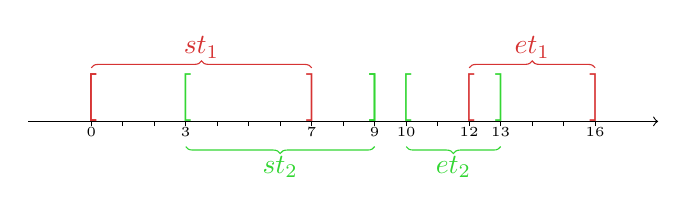
\begin{tikzpicture}
        [decoration={brace},scale=0.4]
        \node (O) at (0,0) {}; 
        \draw[->] (-2,0) -- (18,0);

        \foreach \i in {0,...,16}{
          \draw (\i,-0.15) -- (\i,0);
        }
        \onslide<1-2,4>{  \path (0,0) node[color=red!80!black!80,above=-0.12cm] {\LARGE [} --
          +(0:7cm)node[color=red!80!black!80,above=-0.12cm] {\LARGE ]};}
        \onslide<1,3-4>{\path[green!80!black!80](3,0) node[above=-0.12cm] {\LARGE [} -- +(0:6cm)
          node[above=-0.12cm]  {\LARGE ]};}
        \onslide<1>{ \path[green!80!black!80] (10,0) node[above=-0.12cm]  {\LARGE [}  --
          +(0:3cm) node[above=-0.12cm]  {\LARGE ]}  ;
          \path (12,0) node[color=red!80!black!80,above=-0.12cm] {\LARGE [} --
          +(0:4cm) node[color=red!80!black!80,above=-0.12cm] {\LARGE ]} ; }
        
        \path (0,0) node[below=-0.05cm] {\tiny 0} --
        +(0:7cm) node[below=-0.05cm]{\tiny 7};
        \path (3,0) node[below=-0.05cm]{\tiny 3} -- +(0:6cm)
        node[below=-0.05cm]{\tiny 9};
        \path (10,0) node[below=-0.05cm]{\tiny 10}  --
        +(0:3cm) node[below=-0.05cm]{\tiny 13}  ;
        \path (12,0) node[below=-0.05cm]{\tiny 12} --
        +(0:4cm) node[below=-0.05cm]{\tiny 16} ; 
        

        \onslide<1-2,4>{\draw [decorate,color=red!80!black!80] (0,1.7) -- +(0:7cm)
          node[midway,above]{$st_1$}; }
        \onslide<1>{ \draw [decorate,color=red!80!black!80] (12,1.7) -- +(0:4cm)
          node[midway,above] {$et_1$};}

        \onslide<1,3-4>{ \draw [decorate,green!80!black!80] (9,-0.8) -- +(0:-6cm)
          node[midway,below] {$st_2$};}
        \onslide<1>{   \draw [decorate,green!80!black!80] (13,-0.8) -- +(0:-3cm)
          node[midway,below] {$et_2$};}  
        \onslide<4->{  \draw (0,0)
          node[color=red!80!black!80,above=-0.12cm] {\LARGE [} ;
          \draw[green!80!black!80](9,0) node[above=-0.12cm] {\LARGE ]} ;}
        
      \end{tikzpicture}
    \end{center}
    {\color{gray!60!black!70} \small $2$ tasks $\Rightarrow 4$ events:
      $t_1,\ t_2,\ t_3$ and $t_4$}
  \item<2-> $t_1 \in [0,7]$ \onslide<3->{and $t_2 \in [3,9]$}
    \vfill
  \item<4-> What deduction about $t_2 - t_1$ ?
    
    $t_1,t_2 \in [0,9] \Rightarrow \mathbf{t_2-t_1 \le 9}$
    
  \end{itemize}
  
\end{frame}


\begin{frame}{Maximum separation between events}
  \vfill
  \begin{itemize}
  \item Can be generalized to any pair of events
    \vfill
  \item Can be used as:
    \begin{itemize}
      \vspace{0.2cm}
    \item additional constraints of the model
    \item instead of $M$ in min consump. constraint
    \end{itemize}  
    \vfill
  \item Same reasoning can be used to deduce bound on $t_e$

    {\small \color{gray!60!black!70} {\bf Idea} consider upper bound
      of $[est-i,lst_i]/[eet_i,let_i]$ instead of the whole interval}
    \vfill
  \end{itemize}
\end{frame}


% \begin{frame}
%   \frametitle{Maximum separation between events}
%   \begin{itemize}
%   \item Order the time-window intervals according to:
%     \[ [a,b] \le [c,d]
%       \Leftrightarrow a < c \lor \left( a=c \land b \le d\right)\]
%     \vfill
%     \pause
%   \item Then we have:
%     \[t_{e+1}-t_e  \le   |tw_e \cup tw_{e+1}|    \]
%     \pause
%     \begin{flushright}
%       \textcolor{black!70}{\scriptsize in fact: $t_{e+1}-t_e  \le
%       \overline{tw_e \cup tw_{e+1}} - \underline{tw_e \cup tw_{e+1}}
%       $}
%     \end{flushright}
%     \pause
%     \vfill
%   \item We can use it as:
%     \begin{itemize}
%       \vspace{0.2cm}
%     \item additional constraints of the model
%     \item an upper bound on $t_{e+1}-t_e$ in any constraints using a worst one
%     \end{itemize}
%   \end{itemize}
% \end{frame} 

% \begin{frame}
%   \frametitle{Maximum time for an event}
%   \begin{itemize}
%   \item {\bf Goal: } upper bound on the value of $t_{e}$
%     \vspace{0.4cm}
%   \item<2-> upper bound of each task start and/or end time
%     \vspace{0.4cm}
%   \item<5-> an event must occur before each of these upper bounds
%     \vspace{0.4cm}
%   \end{itemize}
%   \vfill
%   \onslide<3->{
%   \begin{center} 
%     \begin{tikzpicture}
%       [decoration={brace},scale=0.4]
%       \node (O) at (0,0) {}; 

%       \draw[->] (0,0) -- (19,0);
%       \onslide<3>{
%       \draw (1,0) node {\LARGE [} -- +(0:5cm)node {\LARGE ]}; 

%       \draw(4,0) node {\LARGE [} -- +(0:4cm) node {\LARGE ]} ;

%       \draw (8.05,0) node {\LARGE [}  --
%       +(0:6cm) node {\LARGE ]}  ;
%       \draw (12,0) node {\LARGE [} --
%       +(0:6cm) node {\LARGE ]}  ;}
%       \onslide<4>{

%       \draw (1,0) node {} -- +(0:5cm)node {\LARGE ]}; 

%       \draw(4,0) node {} -- +(0:4cm) node {\LARGE ]} ;

%       \draw (8.05,0) node {}  --
%       +(0:6cm) node {\LARGE ]}  ;
%       \draw (12,0) node {} --
%       +(0:6cm) node {\LARGE ]}  ;}
%       \onslide<5>{
%       \draw[color=blue!80!black!50] (0,0) node {} -- +(0:6cm)node {\LARGE ]}
%       node[left,above=0.8cm] {$t_0$}; 
%       \draw (8,0) node {\LARGE ]} ;
%       \draw (8.05,0) node {}  -- +(0:6cm) node {\LARGE ]}  ;
%       \draw (12,0) node {} -- +(0:6cm) node {\LARGE ]}  ;}

%       \onslide<6>{
%       \draw (6,0) node  {\LARGE ]}; 
%       \draw[color=blue!80!black!50](0,0) -- (8,0) node {\LARGE ]} node[left,above=0.8cm] {$t_1$};
%       \draw (8.05,0) node {}  --  +(0:6cm) node {\LARGE ]}  ;
%       \draw (12,0) node {} --  +(0:6cm) node {\LARGE ]}  ;}

%       \onslide<7>{
%       \draw (6,0) node {\LARGE ]}; 
%       \draw (8,0) node {\LARGE ]} ;
%       \draw[color=blue!80!black!50] (0,0) node {}  -- (14,0) node {\LARGE ]} node[left,above=0.8cm] {$t_2$} ;
%       \draw (18,0)node {\LARGE ]}  ;}

%       \onslide<8>{
%       \draw (6,0) node {\LARGE ]}; 
%       \draw(8,0) node {\LARGE ]} ;
%       \draw (14,0) node {\LARGE ]}  ;
%       \draw[color=blue!80!black!50] (0,0) node {} -- (18,0) node {\LARGE ]}
%       node[left,above=0.8cm] {$t_3$};} 

%     \end{tikzpicture}
%   \end{center}
% }
% \end{frame}


% \begin{frame}
%   \frametitle{Maximum time for an event}
%   \begin{itemize}
%   \item Order the time-window interval upper bounds ${\cal UP}$ in
%     increasing order 
%     \vfill
%     \pause
%   \item Then we have:
%     \[t_e \le  {\cal UP}_e\]
%     \vfill
%     \pause
%   \item We can use it as:
%     \begin{itemize}
%       \vspace{0.2cm}
%     \item additional constraints of the model
%     \item an upper bound on $t_{e+1}-t_e$ in any constraints using a worst one
%     \end{itemize}
%   \end{itemize}
% \end{frame}

\subsection{Polyhedral results}


\begin{frame}
  \frametitle{$Z_i$-polyhedron}
  \vspace{0.5cm}
  \onslide<1->{$\rightarrow$ Minimal set of inequalities defining the
    {\it ``$Z_i$-polyhedron''}.}
  \vspace{0.6cm}
  \onslide<2-> {  \begin{block}{$Z_i$-polyhedron}
      form of $z_i \in \{0,1\}^{|{\cal E}|}$ solution? \hspace{2.5cm}
      {\scriptsize (${\cal E}=$event set)}}
    \vspace{0.4cm}

    \onslide<4->{$\Rightarrow$ vector with consecutive-one property  and at least
      one $1$
      \begin{center}
        {\small e.g. $(0,0,1,1,1,0),\ (1,1,1,0,0,0),\ \dots$}
      \end{center}}
    \onslide<5->{     
      \[Z_i= conv\{z_i \in \{0,1\}^{|{\cal E}|} | z_i \text{ of the
          form } (0^*\, 1\, 1^*\, 0^*)\} \] }
    \vspace{-0.2cm}
  \end{block}
  \onslide<3->{\textcolor{black!70}{ \small\[z_{ie}=\left\{
          \begin{array}{ll}
            1 & \text{if task $i$ is in process between $t_e$ and $t_{e+1}$}\\
            0 & \text{otherwise}
          \end{array}
        \right.
      \]}}
\end{frame}


\begin{frame}
  \frametitle{Computational experience}
  \begin{itemize}
    \vfill
  \item Intel Core i7-4770 processor with 4 cores and 8Go of RAM
    \vfill
  \item OS: 64-bit Ubuntu 12.04
    \vfill
  \item MILP resolution: CPLEX 12.6 with 1 thread  
    \vfill
  \item Special separation procedure for non-preemptive cuts ($O(n^2)$)
    for node with depth less than 10 (Preem.)
    \vfill
  \item time limit: 1000 seconds
    \vfill
  \end{itemize}
\end{frame}

\pgfplotstableread[row sep=\\,col sep=&]{
  tasks & Default & Int. & Time & Preem. & I+T+P \\
  20    & 164.14 & 182.2 & 167.3 & 330.9 & 154  \\
  25     & 635.4 & 727.3 & 629.5 & 822.4 & 389.9 \\
  30    & 968  & 851 & 961.4 & 914.8 & 813.8\\
}\mydata

\begin{frame}
  \frametitle{Time comparison for the CECSP}
  \begin{itemize}
  \item Instances of {\it [Nattaf et al.,2015]}
  \item 10 instances of 20, 25 and 30 tasks
  \end{itemize}

  \vspace{0.2cm}
  \begin{center}\begin{tikzpicture}
      \begin{axis}[ enlarge x limits=0.25,
        ybar,
        bar width=.4cm,  
        legend style={at={(0.5,1)},
          anchor=north,legend columns=-1},
        width=\textwidth,
        height=.6\textwidth,
        symbolic x coords={20,25,30},
        xtick=data,
        ymin=0,ymax=1100,
        ylabel={\small time (s)},
        xlabel={\small $\#tasks$}]
        \addplot table[x=tasks,y=Default]{\mydata};
        \addplot table[x=tasks,y=Int.]{\mydata};
        \addplot table[x=tasks,y=Time]{\mydata};
        \addplot table[x=tasks,y=Preem.]{\mydata};
        \addplot table[x=tasks,y=I+T+P]{\mydata};
        \legend{Default, $t_{e+1}-t_e$ , $t_e$ , Preem. , three}
      \end{axis}
    \end{tikzpicture}
  \end{center}
\end{frame}

\pgfplotstableread[row sep=\\,col sep=&]{
  tasks & Default & Int. & Time & Preem. & I+T+P \\
  20    & 90.9 & 90.9 & 90.9 & 72.7 & 90.9\\
  25     &55.6 & 55.6 & 88.9 & 44.4 & 77.8\\
  30    & 10 & 20& 20& 10 &60\\
}\mydat
\begin{frame}
  \frametitle{Solved instances comparison for the CECSP}
  \begin{itemize}
  \item Instances of {\color{gray!50!black!70}\it [Nattaf et al., 2015]}
  \item 10 instances of 20, 25 and 30 tasks
  \end{itemize}

  \vspace{0.2cm}
  \begin{center}\begin{tikzpicture}
      \begin{axis}[ enlarge x limits=0.25,
        ybar,
        bar width=.4cm,  
        legend style={at={(0.5,1)},
          anchor=north,legend columns=-1},
        width=\textwidth,
        height=.6\textwidth,
        symbolic x coords={20,25,30},
        xtick=data,
        ymin=0,ymax=110,
        ylabel={\small $\%solved$},
        xlabel={\small $\#tasks$}]
        \addplot table[x=tasks,y=Default]{\mydat};
        \addplot table[x=tasks,y=Int.]{\mydat};
        \addplot table[x=tasks,y=Time]{\mydat};
        \addplot table[x=tasks,y=Preem.]{\mydat};
        \addplot table[x=tasks,y=I+T+P]{\mydat};
        \legend{Default, $t_{e+1}-t_e$ , $t_e$ , Preem. , three}
      \end{axis}
    \end{tikzpicture}
  \end{center}
\end{frame}



\section{The Discrete Case}
\begin{frame}{Discrete case}
  \vfill
  \begin{block}{DECSP}
    Integer data and solution: Start/End time, Resource reallocation
    time, Resource Consumption.
  \end{block}
  \vfill
\pause
  \begin{itemize}
  \item Constraint Programming Model
    \begin{itemize}
    \item Several types of reasoning (TT, DR, ER...)
    \end{itemize}
    \vfill
\pause
  \item Time-indexed Mixed Integer Linear Program
    \begin{itemize}
    \item valid inequalities deduced from Energetic Reasoning
    \end{itemize}
  \end{itemize}
  \vfill
\end{frame}
\section{General Conclusions and Perspectives}

\begin{frame}
  \frametitle{Conclusion}
  \vfill
  \begin{itemize}
  \item The CECSP is a difficult problem
    \vfill
\pause
  \item Description of properties allowing us to define solution
    methods:
    \begin{itemize}
    \item MILP models
    \item  Hybrid branch-and-bound 
    \end{itemize}
\pause
    \vfill 
  \item MILP model $\simeq<$ Hybrid branch-and-bound
    \vfill 
\pause
  \item Improvement of the MILP:
    \begin{itemize}
    \item 3 sets of valid inequalities
    \item Characterization of $Z$-polyhedron
    \item Improve MILP results for two problems of the literature 
    \end{itemize}
  \end{itemize}
\vfill
\pause
\end{frame}

\begin{frame}
  \frametitle{Perspectives}
  \vfill
    \begin{itemize}
    \item Improve MILP formulations
\pause
      \begin{itemize}
      \item deduce inequalities from CP-reasoning
      \item Strengthening of event-besed model
      \end{itemize}
      \vfill
\pause
    \item Study of the discrete version of the problem
      \begin{itemize}
\pause
      \item solutions are obtained faster  
      \item provide good approximation
      \end{itemize}
      \vfill
\pause
    \item Consider more realistic power processing rate functions
      $f_i$
      \begin{itemize}
\pause
      \item convex functions
      \item concave/convex functions
      \end{itemize}
\pause
    \end{itemize}
  \vfill
\end{frame}

\end{document}






